% REMEMBER: You must not plagiarise anything in your report. Be extremely careful.

\documentclass{l4proj}

\usepackage{amsmath}
\usepackage{amssymb}
\usepackage{adjustbox}

\newcommand{\cit}[1]{\citep{#1}}

\newcommand{\pa}{
	\begin{equation} \label{eq:pa}
		P(A) = \dfrac{n(A) + \dfrac{k}{|\mathbb{A}|}}{\sum_{A \in \mathbb{A}}{n(A) + k}}
	\end{equation}
}

\newcommand{\scoreeqn}{
	\begin{equation} \label{eq:scoreeqn}
		S(C|T) = \sum_{A \in T}{ln\left(\dfrac{P(A) + c\cdot ({I_{A, M}}^\eta + x\cdot {P(A)})}
								 	{P(A)\cdot(1 + c \cdot (\sum_{A \in \mathbb{A}}{({I_{A, M}}^\eta} + x))}\right)}
	\end{equation}
}

\newcommand{\jaccard}{
	\begin{equation} \label{eq:jaccard}
		S = \dfrac{|C\cap{T}|}{|C\cup{T}|}
	\end{equation}
}

\begin{document}

%==============================================================================
%% METADATA
\title{Pep2Path v2}
\author{Ross McBride}
\date{March 27, 2019}

\maketitle

%==============================================================================
%% ABSTRACT
\begin{abstract}

The drug discovery pipeline is an important area of interest for biologists. In particular, natural products are a useful lead for the process of exploring the chemical space, following the evolutionary logic that such products must be useful to the organism that produces them. Recently, the technology of Peptidogenomics was introduced to aid this process by matching mass spectrometry data to gene predictions, allowing us to combine these two sets of information into a better estimator. Pep2Path is a piece of software introduced to automate this matching process, but the original implementation is difficult to maintain in accordance with new developments in bioinformatics. Therefore in this paper we present a software product, Pep2Path v2, aiming to replicate this functionality, and describe in detail both it and the design of this software product. We show that our software implements the main functionality of the original Pep2Path, and is well-tested and reasonably efficient.

\end{abstract}

%==============================================================================

% EDUCATION REUSE CONSENT FORM
% If you consent to your project being shown to future students for educational purposes
% then insert your name and the date below to  sign the education use form that appears in the front of the document. 
% You must explicitly give consent if you wish to do so.
% If you sign, your project may be included in the Hall of Fame if it scores particularly highly.
%
% Please note that you are under no obligation to sign 
% this declaration, but doing so would help future students.
%
\def\consentname {Ross McBride} % your full name
\def\consentdate {27 March 2019} % the date you agree
%
\educationalconsent


%==============================================================================
\tableofcontents

%==============================================================================
%% Notes on formatting
%==============================================================================
% The first page, abstract and table of contents are numbered using Roman numerals and are not
% included in the page count. 
%
% From now on pages are numbered
% using Arabic numerals. Therefore, immediately after the first call to \chapter we need the call
% \pagenumbering{arabic} and this should be called once only in the document. 
%
% The first Chapter should then be on page 1. You are allowed 40 pages for a 40 credit project and 20 pages for a 
% 20 credit report. This includes everything numbered in Arabic numerals (excluding front matter) up
% to but excluding the appendices and bibliography.
%
% You must not alter text size (it is currently 10pt) or alter margins or spacing.
%
%
%==================================================================================================================================
%
% IMPORTANT
% The chapter headings here are **suggestions**. You don't have to follow this model if
% it doesn't fit your project. Every project should have an introduction and conclusion,
% however. 
%
%==================================================================================================================================
\chapter{Introduction}

% reset page numbering. Don't remove this!
\pagenumbering{arabic} 

One particular problem of interest for biologists is the identification of new biological products with novel properties. Until relatively recently, this process was done manually by trained experts. But with the recent advent of the field of bioinformatics, we can now bring immense computational resources to bear on problems like this, saving precious expert time.

\textbf{Pep2Path} \cit{p2p} is a tool that aims to accelerate drug identification by matching mass-spectrometry outputs to identified biosynthetic gene clusters and in the original paper the authors demonstrate robust benchmarking results. However, despite the utility of Pep2Path, it is implemented as a few monolithic scripts, with little room to revise elements of it in accordance with new developments and research without a complete rewrite. In this paper we present a small suite of software tools implementing a platform for functionality like Pep2Path, and the software process by which this software was designed and created.

\section{Aims}

The aims of the project are to:

\begin{itemize}
\item Implement a set of software tools that can achieve similar functionality to the original Pep2Path, subject to correctness testing.
\item Achieve a degree of flexibility in the implementation such that this software can be responsively updated to changes in its environment.
\item Follow good software practises in the implementation such as loose coupling such that we can achieve software reuse, a cornerstone of software development.
\end{itemize}

\section{Motivation} \label{motivation}

Various classes of biological compounds are formed from assembly-chains of smaller compounds, such as \textit{peptides}, which are formed from amino acids.
If we look at this problem as a computer scientist might, the first thing to come to mind in identifying useful drugs within this space might be an exhaustive search of all combinations of molecule.
(Of course, for some molecules questions of topology and structure come into question...)
This quite quickly runs into problems, as with the addition of each component to a chain of biological molecules, the chemical space grows exponentially.
For example, if we consider the relatively limited case of the twenty \textit{proteinogenic} (those involved in the synthesis of proteins, essential for organic life) amino acids and a peptide of length 4, there are \(20^4\) possible combinations... Around 160,000! We would then have to identify which, if any, of these have useful properties.

Without some heuristic (for example being able to infer properties from chemical composition), an exhaustive search of the chemical space is impossible.
Instead we identify biological products produced in the wild, by living organisms - so-called \textit{`natural products'}, which have seen a recent resurgence in study. \cit{natural}
From an evolutionary perspective, we expect that if organisms are expending resources on producing a particular biological product, then it confers a survival advantage.
For example, a strain of bacteria might produce an antibiotic that kills another competitor species of bacteria - which we can then use ourselves to kill a potentially deadly strain of bacteria.
Natural products produced in this way to fulfil an auxiliary function not directly related to the growth or reproduction of the organism are known as \textit{`secondary metabolites'.} \cit{metabolomics}

To identify potentially interesting natural products we could, for example, analyse chemical structure for similarity to other interesting compounds, or by observing similar behaviour across several species which produce a particular product. 
However, we also want to match this natural product to the gene cluster - a Biosynthetic Gene Cluster, henceforth \textbf{BGC} - which encodes it.
One way of achieving this is to cluster together species that share a BGC and produce the natural product in question - this is a good indication that the pattern is meaningful and the BGC produces the natural product.

\textbf{Mass spectrometry} allows us to identify the chemical composition of compounds - by breaking up molecules and then measuring the mass lost, we can infer the \textit{potential} composition of a compound by the masses of its components using a mass-translation table. Mass spectrometry readings, or amino acid \textbf{sequence tags} (short listings of consecutive compounds), are one of the key inputs to Pep2Path. Although there are many classes of natural product for which mass spectrometry can be used effectively, \cit{msomics} here we focus on two particular classes, for which Pep2Path provides an algorithm each: Non-Ribosomal Peptides (henceforth \textbf{NRPs}) and Ribosomally-synthesized and Post-translationally-modified Peptides (henceforth \textbf{RiPPs}). 

The other key input to each of the two Pep2Path algorithms is the gene sequence we are attempting to match our compound to. As their name suggests, RiPPs are synthesised by \textit{ribosomes}, the cell organelle responsible for translating gene sequences to proteins and then modified post-translation by enzymes. As a result, they are precisely encoded in an organism's gene sequence and and we can retrieve their composition directly, as Pep2Path does, by obtaining their \textbf{`six translation frames'} (the six ways the gene sequence can be potentially be read). NRPs, by contrast, are instead synthesised by Non-Ribosomal Peptide Synthetases (henceforth \textbf{NRPSes}) which are independent of the ribosome and can introduce non-proteinogenic amino acids. These consist of several NRPS modules which form an assembly-line of amino acids, and are controlled by three domains - \textit{A (Adenylation)}, \textit{T (Thiolation)} and \textit{C (Condensation)}. Of particular interest to us is the \textbf{Adenylation} domain, which controls which substrate is added to the chain of amino acids. These are not directly encoded into the gene and are therefore harder to predict, so we rely on an external tool - \textbf{antiSMASH} \cit{as4} - for this purpose.

Taking these two sets of inputs, \textbf{NRP2Path} matches the potential chemical compositions generated by mass spectrometry analysis to BGC predictions using antiSMASH, whereas \textbf{RiPP2Path} matches these potential chemical compositions to the six-frame translation extracted from the genetic sequence data of the RiPP-producing BGCs. Pep2Path can then automatically score these two sets of data against one another, filling a key part in an automated drug-identification pipeline, where previously investigation of natural products would be based on hand-identification.

However, the original Pep2Path is written almost entirely using singular scripts, one for each algorithm. As a result, it breaches some important software design principles, by mixing concerns such as parsing input and generating sequence tags, and at times relies on data structures passed around the entire script. This design makes Pep2Path difficult to update, but there are a number of reasons why it might be advantageous to do so. For one, the scoring method the authors use is based on antiSMASH 2.0 \cit{as2} the current version at the time. Since the release of Pep2Path, there have been antiSMASH versions up to 4. \cit{as4} While the original Pep2Path scoring method is backwards-compatible, antiSMASH version 4.0 offers the \textbf{SANDPUMA} ensemble algorithm \cit{sandpuma} which collates the \textbf{Stachelhaus Code} and \textbf{SVM} predictors that antiSMASH 2.0 uses along with several others to offer a more accurate BGC prediction.

Furthermore, we may want to investigate product classes other than NRPS and RiPP, the classes of biological product on which Pep2Path operates - there are many others, including \textit{polyketides} and \textit{alkaloids}. (For an example as to why this might be useful, the pain-medication morphine is an alkaloid extracted from the opium poppy.) It would also be useful to integrate different algorithms for identifying biological products from sequence data (such as the \textbf{RiPPQuest} \cit{rippq} method for \textit{lanthipeptides} - a subtype of RiPP), decouple the mass spectrometry process from the Pep2Path process or otherwise update the scoring mechanism with new developments. We also expect more generally that having a more transparent and modular software design might lead to easier discovery of bugs or integration with other codebases.

%==================================================================================================================================
\chapter{Background}

The motivation for Pep2Path comes from the recent technology of \textbf{Peptidogenomics}. \cit{peptidogenomics} In this original paper the authors propose the method of comparing mass spectrometry sequence tags to translated/predicted genomes for ribosomally-synthesised and non-ribosomally synthesised peptides respectively in order to mine for interesting natural products. However, while there were computational tools for aspects of this process, such as the interpretation of mass spectra and the interpretation of genomes, there was no end-to-end tool automating Peptidogenomics - until Pep2Path. During this section we discuss the background behind Peptidogenomics and Pep2Path, and some of the relevant literature.

\section{Mass Spectrometry}

Mass spectrometry is a common technique in chemistry for the identification of the chemical composition of a molecule by ionising it, causing it to break into fragments. There are multiple approaches to mass spectrometry, and multiple ways to interpret the data - for interpretation, there exist dereplicator tools like \textit{iSNAP} \cit{isnap} and \textit{Dereplicator+} \cit{derep+} which attempt to statistically match mass spectra output to \textit{known} molecules in a database. Dereplicator+ for example, functions by comparing them to sample mass-spectra generated from a known database of chemicals, by simulating how the molecules of those spectra will fragment. 

However, for our purposes we have a series of ordered readings of mass and intensity - gaps in mass peaks correspond to fragmented parts of a molecule, and we can then translate the mass being broken off into a chemical composition using knowledge of molecular weights stored in a dedicated mass translation table. (The so-called \textit{`de novo'} mass spectrometry technique - alternative methods are an active area of research.) Traditionally, this was a problem hand-solved by chemists, but has long been a target for computational processes due to the ease of translation of these numerical processes. 

Once mass shifts have been translated to potential compounds, these can be joined together, end-to-end into longer sequences of compounds - `sequence tags'. Then, computational resources can be used to easily mine a group of mass spectrometry readings for sequence tags. However, there will inevitably be noise in mass spectrometry readings, whether from measurement error or the breaking off of small fragments that don't represent a significant part of the molecule. For this reason, two variables are introduced: an \textit{intensity threshold} and a \textit{mass tolerance}. We can firstly cut out all low-quality readings by cutting out all readings below a certain intensity; secondly, we can account for slight discrepancies in mass measurements by measuring mass shifts within some interval rather than taking the exact values from the mass table. Good values for these variables depend on the dataset in question, and a good general pair of values is currently unknown, but processing mass spectra in this way is standard across most approaches.

\section{BGCs}

\subsection{NRPs and antiSMASH}

antiSMASH (antibiotics and Secondary Metabolite Analysis Shell) \cit{as4} is a widely-used piece of bioinformatics software used for the automated labelling of BGCs and genome-mining of secondary metabolites from raw sequence genome sequence data extracted from bacteria, fungi or plants. It is usable both as a standalone program on MacOS or Linux and as a web-server and has gone through several revisions and is, at the time of writing, currently up to version 4.0. Therefore, it aggregates many of the latest developments in natural product research and offers many features for the handling of such sequence data and the annotation of its BGCs, outputting data in the standard GenBank format.

For the purposes of this paper, we are interested in antiSMASH's ability to predict the substrate specificity of an NRPS' adenylation domains, that is, give us a prediction for the chemical makeup of a particular NRP given the sequence data of the organism that produces it. The current version of antiSMASH uses the SANDPUMA ensemble algorithm to do this, which aggregates the results of several other predictive algorithms, including those in previous versions of antiSMASH (maintaining backwards-compatibility), to produce significantly better results. However SANDPUMA and antiSMASH 4.0 are relatively recent compared to Pep2Path, and instead we are interested in two key predictors of antiSMASH 2.0: the Stachelhaus Code, a set of rules for comparing different adenylation domains created from empirical observation \cit{stachelhaus} and a machine learning Support Vector Machine (SVM) based method.

Machine learning is frequently used in bioinformatics to extrapolate underlying trends from the vast quantities of data often involved, learning from a provided dataset useful understandings of programmer-selected features by performing some optimisation task. SVMs in particular are a classifier (that is, assign inputs to one of a set of discrete classes, in this case a substrate prediction) and attempt to draw a decision boundary separating those classes so as to minimise the distance between a certain number of the training datapoints plotted in a hyperplane. The SVM implementation for antiSMASH is provided by \textbf{NRPSPredictor2}, \cit{nrps2} a standalone piece of software which has since been integrated into the antiSMASH pipeline. One of the the things that makes the original Pep2Path results robust is that it was tested on datasets NRPSPredictor2 had \textit{not} been trained on, avoiding the introduction of bias and showing the generalisability of the Pep2Path method.

\subsection{RiPPs, their six-frame translation and RiPPQuest} \label{ripps}

For RiPPs, the translation process is more direct than with NRPs, and does not require an external platform like antiSMASH to make substrate predictions. This process can be done via the `six-frame translation'. DNA strands are made of long strings of four \textit{nucleobases} \textit{(Adenine, Glycine, Thymine and Cytosine)} which can easily be represented and processed in computer systems in large numbers, and which bind in A-T and G-C pairs across the two strands. These bases, in groups of three known as \textit{codons}, reliably encode amino acids in ways we can extract. However, when looking at a genome, we do not know where the first codon begins - it could begin at any of three positions. Then, the encoding could be done by either strand - we only store one strand, but we can retrieve its \textit{reverse complement} by converting the base to its corresponding base and reversing the strand - for a total of six different encodings. This is the six-frame translation method we use for RiPPs.

Among RiPPs, there are many subtypes. One particular subclass of interest is the lanthipeptide, which is specifically targeted by the bioinformatics software RiPPQuest. \cit{rippq} A successor to the original Peptidogenomics paper, the RiPPQuest method centres on the prediction of the \textit{`LANC-like'} domain in the genome, which is important for the biosynthesis of lanthipeptides in particular. It then centres its translation window around the LANC-like domain and begins searching using the six translation frames. 

One particular note is that as sequence data gets larger, so will the probability of random matches to our sequence tag. This method's performance improves as we have either longer sequence tags, or shorter sequence data. If we assume (as a purely illustrative exercise) that there is uniform probability for each sequence tag across the chemical space, for the 20 proteinogenic amino acids (the alphabet for RiPPs) then the probability of any given sequence tag of length 2 is \(\dfrac{1}{400}\). Relatively likely, even in small data. However, a peptide of length 4 would have the probability \(\dfrac{1}{160000}\). Of course, longer genome sequences may contain enough data to appear to have several million peptides and \textit{still} randomly match tags of length 4, 5 or even upwards, but it gets exponentially less likely as sequence tag length increases.

One of the motivations for RiPPQuest is that lanthipeptides have relatively short sequence tags, and thus it is necessary to target the sequence length. By targeting the translation window around a LANC-like domain, RiPPQuest searches less of the genome and provides more accurate results, but consequently only operates on lanthipeptides in particular. (These are some of the features relevant for comparison to our method - there are other complexities to their method which we will not remark on here.) We do not implement the RiPPQuest method here, and instead implement a more general method with looser assumptions in order to target all classes of RiPP, but we highlight this method as a point of comparison and possibility for future extension.

\section{Pep2Path}

Pep2Path \cit{p2p} provides two algorithms, NRP2Path and RiPP2Path. Both rely on the same principles of mass spectrometry. In the original Pep2Path source program, mass search tags can either be given directly or can be derived from a mass-shift sequence. They then extract relevant BGC information from a sequence, and compare potential sequence tags to potential BGCs using a different scoring function for each algorithm in order to enable finding the best match.

\subsection{NRP2Path} \label{nrpbackground}

NRP2Path first takes potential sequence tags and antiSMASH substrate specificity predictions. These sequence tags can be arranged either forwards or backwards, and within the prediction there are several different NRPS modules, which themselves can either be arranged forwards or backwards and can be arranged in any order to make up the full BGC sequence. So in order to test all possible gene sequences, Pep2Path must generate all permutations of the cartesian products of the forwards and backwards modules (a total of \(n!\cdot2^n\) different orderings for \(n\) modules). A sequence tag and an ordering of a gene sequence are then aligned with one another and scored for their match, testing every possible alignment in order to find the best score.

\begin{figure}
    \centering
    \makebox[\linewidth][c]{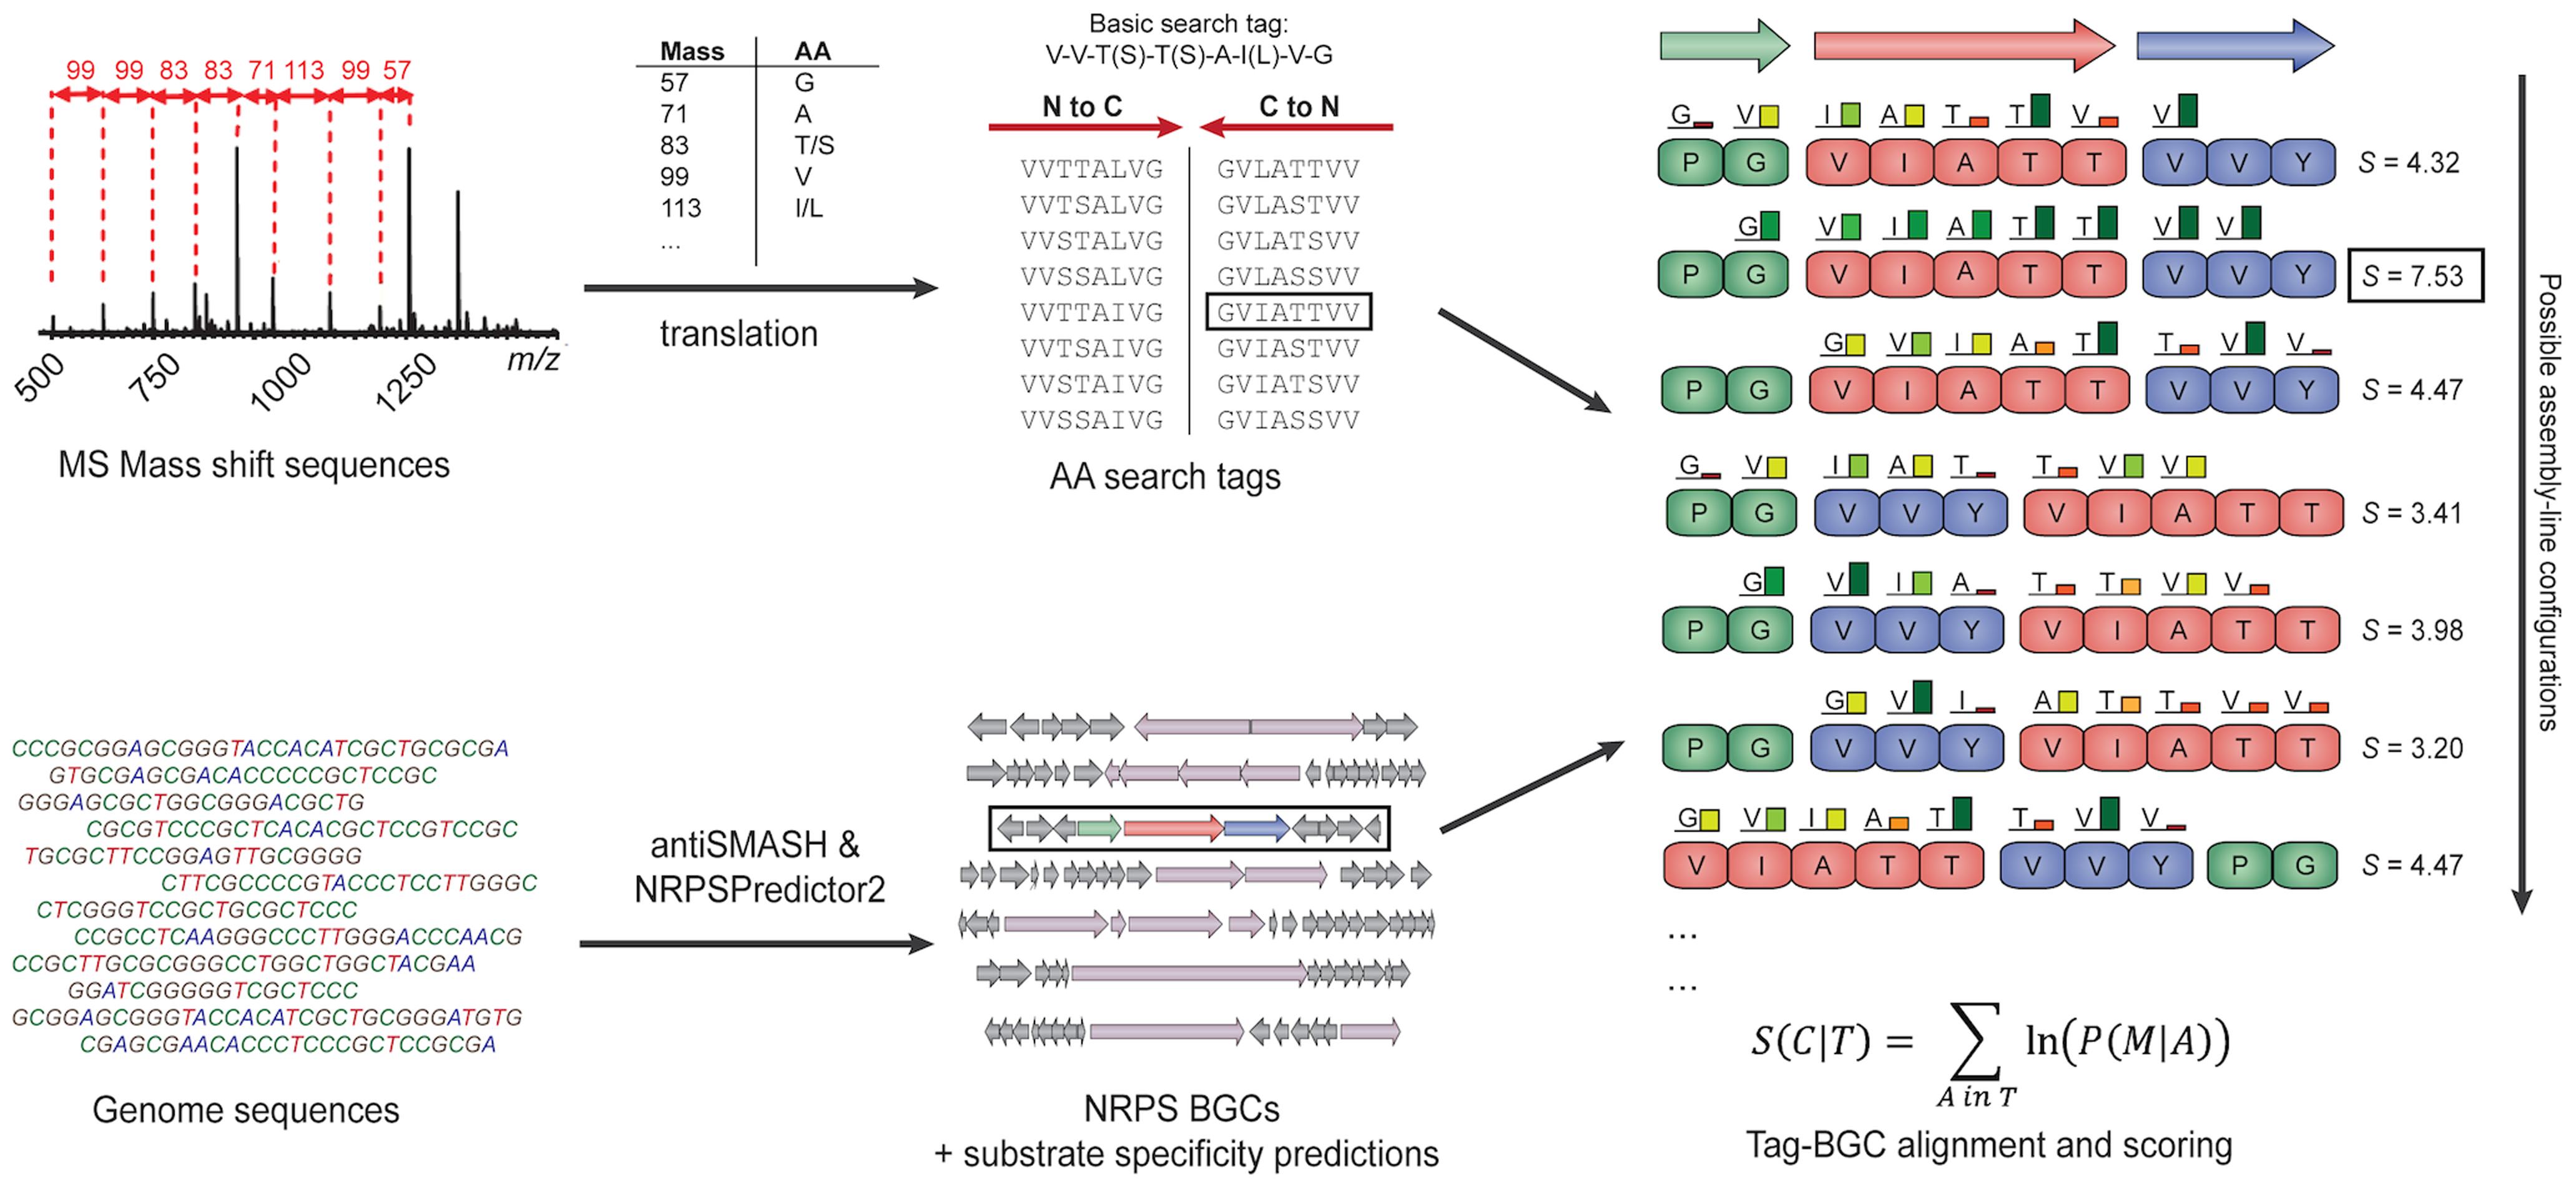
\includegraphics[width=1.25\linewidth]{images/nrp2path.png}}%

    \caption{An illustration of the NRP2Path algorithm. On the top is a mass spectrometry output being put through a mass translation table to produce
    a comprehensive list of potential sequence tags. On the bottom is BGC substrate specificity being extracted from raw sequence data by antiSMASH.
    These two sets of data are then used to compare every alignment of every sequence tag to every possible ordering of NRP blocks extracted from the 
    BGC. using the abbreviated scoring function shown below. Figure adapted from \cite{p2p}.
    }

    \label{fig:nrp2path}
\end{figure}

In order to compare a sequence tag to a BGC, NRP2Path uses its own scoring function loosely inspired by \textit{Bayes' Rule}. We omit the details of its derivation here for brevity's sake, but they are available in the original paper.

\scoreeqn

\(S(C|T)\) is the score of a gene cluster given the sequence tag. \(A\) is the amino acid making up part of a tag, and \(\mathbb{A}\) is the total amino acid alphabet being used. \(c\) and \(x\) are parameters that express the degree of confidence that final probability relies on substrate specificity rather than prior probability, and a pseudo-count to correct for small sample size, with default values \(c=1\) and \(x=0.01\), respectively. \(\eta\) is a regularisation term allowing for the exponential penalisation of repeated mismatches. \\

\(I_{A, M}\) is the average of two values calculated separately for the Stachelhaus Code and SVM predictions. The Code prediction is based on the closeness to the closest known NRPS module for NRPSPredictor2, whereas the SVM value is assigned between five evenly-spaced thresholds between 0 and 1 based on how closely the classes of the amino acid match (0 for no relation, 1 for exact match). \\

\(P(A)\) is the prior probability of \(A\), calculated like so:

\pa

where k is another pseudocount with k=1 and n(A) is the number of appearances within the NORINE database. \cit{norine}

Finally, the degree of matching between any gene sequence and mass spectrometry output is defined as the maximum of its scores across any alignment.

\subsection{RiPP2Path}

While RiPPQuest provides a method for the matching of BGCs to mass spectrometry readings in lanthipeptides, it does not cover all RiPPs. Following RiPPQuest, Pep2Path introduced RiPP2Path, a simple accessory tool for more broad matching of RiPPs. It functions by running a sliding window containing the sequence tag over every position of every translation frame in a gene sequence, computing the number of amino acid matches over the total length of the tag and then returning the highest scores.

Unlike RiPPQuest, this algorithm is naively targeted and processes a score for each gene subsequence, distinguishing them only by the score they receive. This does have penalties for accuracy where any identified sequence is more likely to have have appeared purely by random chance, especially in larger data, and costs more processing power inasmuch as it searches more, but it comes with the benefits of a very simple algorithm and is capable of applying the technology of peptidogenomics to all classes of RiPP, not just lanthipeptides.

%==================================================================================================================================
\chapter{Analysis/Requirements}

In this section, we lay out the exact motivation for various proposed requirements of the software and their priority, and then go on to list these formally.

\section{Problem Analysis}

For this project, the supervisor acted as a client, proposing the software for eventual integration into a larger codebase, and due to greater domain experience provided requirements implicitly as the project progressed. 

Firstly, we wanted a set of tools to implement the original Pep2Path functionality. This meant implementing NRP2Path and RiPP2Path. Secondly, the client had their own dataset for which the alignment comparison of NRP2Path might prove particularly cumbersome. This then meant being able to read the formats of the data available, and implement a simpler algorithm comparing the overlap between components. We also desired these implementations to be flexible with respect to future advances in bioinformatics and allow the integration of custom scoring functions, and to, as far as possible, allow space for future algorithms for other chemical classes to be implemented within the same framework, as we outlined in the introduction. (\ref{motivation}) We implement both of these described NRP-comparison algorithms both to solve the more proximal problem of extracting useful information from the client's dataset, and also to demonstrate the flexibility of our implementation and its potential for various algorithms to be incorporated within. Note however that while we also follow this procedure for scoring functions (i.e. we implement a trivial scoring function and the original Pep2Path scoring) producing a more up-to-date scoring function - for example one that takes advantage of the SANDPUMA predictor - is a research endeavour unto itself and is outwith the scope of this project - we only aim to provide a \textit{platform} for more modern techniques.

Furthermore, for Pep2Path to function, it requires both the previously-mentioned mass spectrometry and biological inputs to function. Logically, then, the software must be able to source this input from somewhere. Where the A-domain predictions are concerned, we outsource this work to antiSMASH as the original Pep2Path does - it is well-maintained and the leading piece of software in this area. Additionally, the client's data was already in antiSMASH-produced Genbank form - although this also contains the raw sequence data, accurately predicting A-domains is a problem unto itself, and entirely outside the scope of this project. Where RiPP2Path is concerned, it only takes raw sequence data - so in both cases, on the gene side of things, the software needs only parse antiSMASH-generated Genbank output.

Mass spectrometry, however, is more complicated. We have data from mass spectra, but not sequence tags. This obviously creates a requirement to derplicate these spectra. However while this problem has been thoroughly studied (and continues to be thoroughly studied) and has an incredible breadth of software solutions available, the breadth of such solutions presents a challenge in itself, and hitherto much of the field has focused on protein-identification, \cit{msomics} as seen in software such as Mascot. \cit{mascot} Rather than trying to find a tool that best fits our needs, we instead propose that the software should have a simple \textit{de novo} mass spectrometry algorithm, focusing on no specific mass table, and usable for any peptide sequence. This violates the software engineering principle of software reuse, but eliminates the need for biochemistry research as a prerequisite, and potentially issues with of software licensing, allowing us to package Pep2Path as a standalone piece of software, with only the open-source antiSMASH as a dependency. Additionally, we can mitigate the effect of `reimplementing the wheel badly' by having a modular structure such that the mass spectrometry component can be replaced by any implementation an interested party thinks would suit their use-case and the only real drawback in this case is processing speed.

The software has to handle some very large search spaces, so efficiency \textit{is} a concern. However, the client had a preliminary stage of screening for data reducing the data our implementation would have to process. Additionally, it would also be run on powerful hardware dedicated to processing very large bioinformatics data, so whilst it was necessary for our implementation to be efficient enough to terminate in reasonable time (and not, say, have unnecessary orders of complexity included within algorithms), the absolute highest degree of efficiency was not an aim for this project. Particularly, we are interested in a reasonable running-time for \textit{Pep2Path}. This means not concerning ourselves overly with the efficiency of the mass spectral sequencing - for which efficient algorithms are a separate subfield of study.

It is also important to note that RiPP2Path, while it is a desirable inclusion, is a rather simple accessory tool and is lower-priority than a full implementation of NRP2Path - the highest priority is to deliver an end-to-end \textit{flexible} implementation of NRP2Path to the client, and preferably, implement it in the client codebase, but the simplicity of RiPP2Path also makes it an easy inclusion. Some other useful features to include are (in descending order of significance); the ability to compare a group of spectra to a group of genomes and return some group-matching statistics; an accessory tool to plot the mass spectrum and visualise an identified sequence tag along it; and a CLI in order to run the program as a standalone application.

Moreover, while the full method of RiPPQuest for collecting RiPPs from a genome is its own algorithm, orthogonal to anything we are implementing here, and we leave the complexities of this method to software like RiPPQuest - however, it might be possible, and relatively simple, to use the basic idea of restricting the genome to a subsection around a LANC-like domain for a lanthipeptide, offering faster and less noisy predictions for this specific case of RiPP2Path with a simple alteration to the algorithm.

While the top priority is to deliver functional software to the client, we also wish to contribute to the bioinformatics ecosystem more broadly. One of the major issues facing bioinformatics research is the necessity of two different fields of domain-specific knowledge - biology and computer science, and their associated subfields (organic chemistry, software engineering...). Although attempts are being made to more broadly disseminate the domain-specific knowledge necessary, \cit{msomics} solving these issues will likely require interdisciplinary efforts. Then for our software to \textit{meaningfully} contribute to the bioinformatics ecosystem, it should be accessible to outside experts. This means a clear and transparent design, and to use the established software tools where we use tools. Additionally, in order to be as accessible as possible, the software should be as platform-independent and as portable as possible. 

These are some more advantages of using a simple home-brewed MS package in lieu of trying to find a specific tool - a lack of dependencies makes Pep2Path easier to configure and get started, and the design should be (in theory) clearer to an observer, especially when compared to proprietary software. antiSMASH, our only external dependency, is only supported for Linux and MacOS, but our intent is to rely on its output files rather than the software itself, where these files can be produced either on a compatible system, or by the web server version. End-users should be concerned as little as possible with the configuration of the software on their system.

Finally we wish to deliver a software that we can \textit{demonstrate} to be correct, and provide a baseline for which future additions to it can be measured against. For this reason we implement unitary testing across our implementation, where we demonstate adherance to some invariant that should in principle guarantee the implementation correctly maps from the design. As a practical test, to prove that scoring functions meet our expectations, we also implement some tests on synthetic - known - data to see if our scoring functions behave as we would expect. We additionally would preferably have software that can replicate the original experimental results of Pep2Path using the datasets they provide; this would allow us to show both that our implementation of the Pep2Path scoring mechanism was correct, but also that we have provided a platform that supports scoring functions such as Pep2Path's scorer.

\section{Requirements} \label{moscow}

In this section, we list functional requirements using the MoSCoW method, and then non-functional requirements as their own following list.

\subsection{Must Have}

\begin{itemize}

\item A simple \textit{de novo} mass spectrometry tool capable of converting mass/intensity readings to sequence tags.
\item Various small tools to be able to read in input data from standard file formats. Particularly, the ability to read the domain-standard antiSMASH-produced Genbank file formats.
\item A software base allowing the integration of custom scoring functions, and allows the provision of custom mass tables/alphabets for the compounds being operated on, with a simple scoring method and the original NRP2Path scoring method implemented to demonstrate its capacity in this regard.
\item Implementation of a simpler BGC/mass-spectrometry comparison equivalent to taking the set overlap of the components in both, more suited to datasets with shorter sequence tags.
\item A full implementation of NRP2Path.
\item A suite of unit tests verifying the behaviour of the implementations of the various algorithms and improving future maintainability.
\item Practical tests showing the behaviour of the scoring function.
\end{itemize}

\subsection{Should Have}

\begin{itemize}
\item Integration with the client's codebase.
\item A full implementation of RiPP2Path.
\item The ability to run a `many-to-many' comparison between BGC-predictions and mass spectrometry.
\item Replications of the original experimental results for Pep2Path (not necessarily exact, but on-target) to demonstrate functional correctness by practical test.
\end{itemize}

\subsection{Could Have}

\begin{itemize}
\item An accessory visualisation tool to plot mass spectra with predicted sequence tags over them.
\item A simple CLI to run as a standalone.
\item An adaptation of the RiPPQuest method to narrow down the translation down to just the region around the LANC-like domain for lanthipeptides.
\end{itemize}

\subsection{Won't Have}

\begin{itemize}
\item Implementations of novel scoring functions, such as one that takes advantage of antiSMASH 4's use of the SANDPUMA ensemble.
\item A full implementation of the RiPPQuest method for genome mining on lanthipeptides.
\item Any attempt to predict A-domains - this should be left to antiSMASH.
\end{itemize}

\subsection{Non-Functional Requirements}

\begin{itemize}
\item Should maintain strong separation of concerns and loose coupling, so components can be reused.
\item Platform-independence (portability).
\item Transparency of design.
\item Reasonable efficiency - not a priority, especially where MS-sequencing is concerned, but the software should avoid wasting time where possible.
\item Accessible to outside experts - using established tools where it is necessary to use tools.
\end{itemize}

%==================================================================================================================================
\chapter{Design}

In this section, we lay out the high-level design features of the software, prior to any implementation details, describing both a proposed architecture and the algorithms used.

\section{Software Structure}

Examining our proposed software, we partition it into a design separated along a structure much the same as the one we have been describing Pep2Path in. There are three important concerns: mass spectrometry, sequence handling, and the implementation of the two Pep2Path algorithms themselves, reliant on the two prior concerns. Therefore we propose a design to separate our software into corresponding packages along these lines. 

\begin{figure}
    \centering
    \makebox[\linewidth][c]{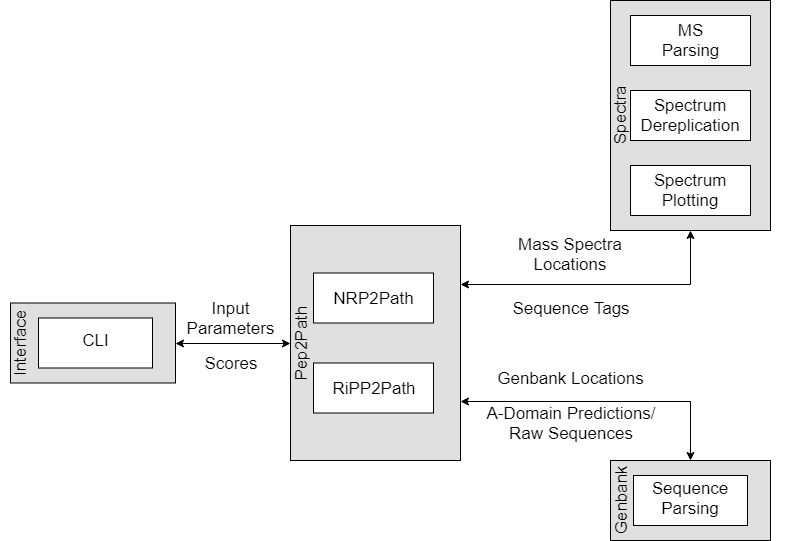
\includegraphics[width=0.9\linewidth]{images/system_layout.png}}%

    \caption{An illustration of the largest version of our proposed system layout. The CLI and Spectra Plotting are not as high-priority as the other
    components. We write input on the top of arrows, and output on the bottom.
    }

    \label{fig:system_layout}
\end{figure}

One module must handle the parsing of any relevant MS data file formats from our client's data, the extraction of sequence tags from such data and a possible accessory tool to plot the sequence tag along its corresponding spectrum. Another must handle the extraction of useful information from sequence data - that is, adenylation domain predictions and raw sequence data from antiSMASH-produced Genbank files, for NRP2Path and RiPP2Path respectively. Finally, the last module must have both of these as dependencies, receiving sequence tags from the spectra module and A-domain predictions and raw sequence data from the Genbank module, and then implement NRP2Path and RiPP2Path. Then, each of these modules should have its own set of tests. Additionally, if a standalone CLI were to be implemented, this would then wrap around the outside of the software, treating the entire Pep2Path and its dependencies as its own dependency.

This design permits us to separate our implementation of the Pep2Path algorithms from the data fed into them, whilst still providing an end-to-end implementation from raw MS data and antiSMASH data to match scoring. For example, one would be able to entirely remove the MS package, replace it with another that provides the same interfaces and sequence tags as output (perhaps using a different algorithm for MS-sequencing) and Pep2Path should function unchanged.

\section{Algorithms} \label{algorithms}

During this section, we describe precisely the various algorithms we use for this project - note that for MS-sequencing and NRP2Path, we do not specify a mass table/alphabet respectively, and allow the user to provide this. In the case of mass spectra this is totally context-dependent on the molecules being fragmented - in the case of NRP2Path, different predictors may use different alphabets, and so different alphabets will be provided implicitly with the provision of different scoring functions.

\subsection{Mass Spectra Sequencing} \label{msalgorithm}

The input to the \textit{de novo} mass spectrometry algorithm is a list of mass spectrometry readings, each with a mass value and an intensity value, where mass gaps represent a potential compound. We then want to convert these values into all potential \textit{sequence tags}, end-to-end lists of possible components. (That is, in a sequence tag, each component must have its gap begin where the previous gap ended.) 

Therefore, first, we preprocess our peaks to remove all low-intensity readings, according to some user-chosen threshold (perhaps 5\% of the maximum value in a spectrum, for example), and sort them so that they are increasing order of mass. We then want to find gaps in the masses that correspond to the masses in some table of compounds (with some tolerance, either percentile or absolute) and find all end-to-end sequence tags from this.

We can formally model this problem as a \textbf{DAG} (Directed Acyclic Graph), a digraph with a topological ordering - that is, each vertex is enumerated and vertices can only have edges to vertices with higher numbers.  (There may be multiple topological orderings - for example consider the case where there are multiple \textit{sources} - nodes with no ingoing edges - in the graph. Either could be labelled as the first node! We specifically use an ordering by increasing mass and direct edges towards higher masses, labelling from \(1\) to \(n\).) Furthermore, edges have a label, which is a list of all potential compounds that could be between the peaks the vertices represent, and these edges and their labels are unknown, but discoverable. In this model, vertices are individual mass spectrometry readings (mass and intensity), and edges are potential compounds from gaps between mass peaks. The problem of finding a sequence tag then corresponds to finding a path through this graph. \cit{msbook}

\begin{figure}
    \centering
    \makebox[\linewidth][c]{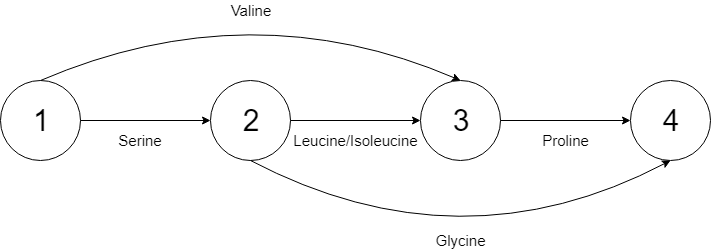
\includegraphics[width=1.0\linewidth]{images/peak_graph.png}}%

    \caption{An example illustration of some mass spectra peaks represented as a DAG, with arbitrarily chosen amino acid names for the edges. From this 	    graph there would be the tags (without subtags) Ser-Leu/Ile-Pro, Val-Pro, Ser-Gly.
    }

    \label{fig:peak_graph}
\end{figure}

We partition this algorithm into two stages: \textbf{edge discovery} and \textbf{path discovery}. Edge discovery is the process of searching the raw numerical mass values of each peak for gaps corresponding to components in the mass table, in order to build the graph's edge set. Path discovery is then traversing the edges in the edge set in order to form a complete path - and therefore a sequence tag.

To perform edge discovery, we begin by allowing a value to be specified for a mass tolerance. This might be a static value measured in \textit{Da} (Unified Atomic Mass Unit or Dalton), a percentage applied to each mass in the mass table, or a percentage of the maximum mass in the spectra readings. First we iterate through the indices of mass peaks; for every mass peak, we subtract its mass value from the mass value of subsequent peaks, to create a table of mass differences. We then iterate through every compound in the mass table, first transforming its mass into an interval \((mass - mass\_tolerance, mass + mass\_tolerance)\) and then checking every mass difference to see if it lies within these bounds. If a mass difference \textit{does} lie within the interval, then an edge exists between the peaks with a label corresponding to the compound from which we made the interval. We repeat this for all values in the mass table in order to find all possible edges.

\begin{algorithm}
    \DontPrintSemicolon
    \KwData{$v$ A collection of pairs of mass, intensity readings. \;
		 $mt$ A mass-tolerance. \;
		 $it$ An intensity threshold. \;
		 $mass\_table$ A table of compound masses}
    \KwResult{$E$ A labelled list containing all edges between vertices and their labels}
    \Begin{
	$E \leftarrow \{\}$\;
	$n \leftarrow |v|$\;
	$v \leftarrow filter\_by\_intensity(v, it)$\;
        $v \leftarrow sort\_by\_mass(v)$\;
	\For{$1 \leq i \leq n-1$}{
		$md \leftarrow []$\;
		\For{$i \leq j \leq n$}{
			$md[j-i] \leftarrow v[j] - v[i]$\;
		}
		\For{$label, mass \leftarrow mass\_table$}{
			$minm, maxm \leftarrow (mass - m, mass + mt)$\;
			\For{$i \leq j \leq n$}{
				\If{$minm \leq md[j] \leq maxm$}{
					$E[i] \leftarrow (j, label)$\;
				}
			}
		}
	}
    }

\caption{Edge Discovery Algorithm}\label{alg:edgedesc}
\end{algorithm}

To perform path discovery, we perform an exhaustive depth-first search for every peak in the vertex set. (A breadth-first search would also be possible but depth-first is conceptually simpler to understand.) First, we choose a vertex, and denote it as our current vertex. So long as our current vertex has edges we haven't yet explored, we choose one of those edges, marking it as explored, and make the other vertex involved in the edge our current vertex and push our previous vertex onto a stack. We continue this process until we reach a vertex with no unexplored edges. At this point we pop the vertex at the top of our stack, marking it the new head as our current vertex and resume searching for edges. Once we have also exhausted our stack, we choose another vertex we have not already performed this process for, and repeat until we have exhausted all vertices, to get all possible sequence tags.

There are a few obvious optimisations we can make on this process: firstly, we do not need to check for cycles as we normally might in our depth-first search, as by definition our DAG has no cycles. Secondly, the solution space for our tags is very large - \(\sum_{len=1}^{n}{alphabet\_size^{len}}\) specifically, for all tags up to length \(n\), ignoring for now how these tags might be arranged along our peaks. Rather than storing each tag as we find it, we can instead store the longest tag containing this tag as a substring (we refer to such substrings as \textit{subtags} or here). 

This is done for two reasons: under normal circumstances, we assume if we have found an edge, then unless the data is exceptionally noisy the edge itself is likely meaningful, and furthermore any subtags can be reconstructed by taking n-grams of the parent tag. For each parent tag, this saves us having to store \(\dfrac{n}{2}(n+1)\) subtags. (Consider that a sliding window of length \(m\) has \(m-n+1\) possible alignments across a sequence tag of length \(n\), and that we wish to consider the sum of all \(1 \leq m \leq n\) and apply the standard formula for the sum of an arithmetic sequence.) For our algorithm, this means saving a sequence tag \textit{only if} we have exhausted all edges and we haven't just popped something from the stack. Finally, if we visit a vertex as part of path discovery for another vertex, there is no need to begin a tag search beginning from that vertex - any tags discovered this way would be subtags of the tags we have already discovered.

\begin{algorithm}
    \DontPrintSemicolon
    \KwData{$E$ A labelled list of edges, containing all edges between vertices and their associated labels}
    \KwResult{$T$ The set of all tags (paths) discovered, with no subtags}
    \Begin{
	$T \leftarrow \{\}$\;
	$skip \leftarrow \{\}$\;
	$s \leftarrow []$\;
	$lastop \leftarrow false$\;
	$n \leftarrow size(E)$\;
	\For{$1 \leq i \leq n$}{
		\If{$i \in skip$}{
			go to next $i$\;
		}
		append $i$ to $s$\;
		\While{$size(s) > 0$}{
			\While{$\exists unexplored\_j \in E[s.head]$}{
				mark edge $\{i, j\}$ as explored\;
				append $j$ to $skip$\;
				append $j$ to $s$\;
				$lastop \leftarrow true$\;
			}
			\If{lastop}{
				append $s$ to $T$\;
				$lastop \leftarrow false$\;
			}
			pop from $s$\;
		}
	}
    }

\caption{Path Discovery Algorithm}\label{alg:pathdesc}
\end{algorithm}

Where theoretical performance is concerned, we expect edge discovery to be \(O(n^2)\): calculation of mass differences is \(i-1\) operations for some mass peak \(0 < i < n\) and this process will be performed \(n-1\) times; arithmetic sum gives us \(O(n^2)\) complexity. (The number of masses in the table is another multiplicative factor, but is effectively constant.) For path discovery, we shall not formally prove its complexity bound here (this is not the focus of this work), but we shall give a rough illustration: suppose there are edges between every peak and its subsequent peaks. (This is an unrealistic assumption in practise - this would suggest there is more noise than actual data!) Then it is possible to construct exactly one path of length \(m\) by choosing any \(m\) peaks from the whole set of \(n\) peaks. Therefore the number of paths must be \(\sum_{m=1}^n\binom{n}{m} = 2^{n} - 1\) - exponential in number of solutions. \footnote{This is a special case of the binomial theorem, \(\sum_{m=0}^{n}\binom{n}{m}x^{m}y^{n-m} = (x+y)^n\). Set both \(x\) and \(y\) to \(1\) and we have \(\sum_{m=0}^{n}{\binom{n}{m}} = 2^n\). Then subtract \(\binom{n}{0} = 1\) for \(\sum_{m=1}^{n}\) therefore \(2^n - 1\).} 

However, for our restricted version where we do not consider subpaths, then consider that each \(m^{th}\) vertex may have a path to any of its subsequent \(m-1\) vertices. Normally, whenever we add an edge like this, it would double the number of paths: for each path beginning at a vertex \(m\) with an incoming edge from vertex \(m'\), there would be another path beginning at \(m'\) and passing through \(m\). However, under our restriction, this second set of paths begins at \(m'\) is the only set counted: since it has an equal number of paths, this means that when we traverse an edge from one node to another node that has paths already in our 'path-set', and update this 'path-set' accordingly -- the number of paths remains constant. The only time the number of paths in the path-set increases under this restriction is when a node connects directly to a terminal node -- otherwise there exists subpaths that we are extending and therefore replacing by this process. Then for each node its number of paths with no subpaths is the number of terminal nodes which follow it; since in the worst-case, non-terminal nodes and terminal nodes can be understood as a function of the total number of nodes \(n\), under this simplifying assumption this part of the algorithm should be \(O(n^2)\). \footnote{This maps cleanly onto an inductive proof.} (Alternatively, one can represent this problem as linear with the number of edges, but number of peaks is known \textit{a priori} whereas edges are not, so we choose to represent it by number of peaks.)

Therefore, under our simplifying assumption, we have \(O(n^2)\) complexity for the solution space of the path discovery problem (this maps directly onto our time-complexity since there is a one-to-one correspondence between the edges we traverse) as long as we only have one element in the mass table (not a very useful assumption). However, in noisy data, any path may still have up to \(alphabet\_size\) labels, and therefore up to \(alphabet\_size^n\) variations of the path for different labels. This is a very pessimistic estimation unless every mass in the table is very close together or the mass-tolerance is set unreasonably wide, but if masses are close then this can very quickly become problematic without necessarily coming close to this worst-case scenario. Leucine and Isoleucine have identical masses: so, purely for the sake of illustration, if we were to chain ten of these, there would be \(2^{10} = 1024\) possible tags for one exact set of data. For Leucine and Isoleucine we chose to represent them as a single tag in our table when we used them in order to avoid this issue but this is something worth noting for noisy data, and mass tables with similar masses contained within.

However, note again that this is a relatively naive solution to a well-established problem. We include it here so as to have a complete, end-to-end software pipeline for NRP2Path, but due to our proposed modular structure, it would be relatively easy to replace it with another, more sophisticated mass-spectrometry module and still take advantage of Pep2Path. For example, some approaches include: using a scoring mechanism to measure the fit between a predicted sequence tag and the real data during edge discovery, eliminating impossible sequences early or by completely different approaches such as optimising a scoring function over the entire scoring space using a genetic algorithm or using a Hidden Markov Model. \cit{protointro}

However, perhaps most interestingly, one approach that has been used for quite some time is to construct a scoring graph and attempt to solve an instance of the \textit{Antisymmetric Longest Path Problem}, an NP-Hard problem that is a variation of the \textit{Longest Path Problem}, (the classical problem of finding the longest path in a graph, also NP-Hard). \cit{protobook} (And therefore under the assumption that our result is not generated by noise, that it returns the true value.) Recent work suggests both tighter bounds on the problem (and its inapproximability) \cit{alppbound} but also that under certain restrictions, a linear-time algorithm may be applied to solve the antisymmetric path problem (and particularly, has been tested on spectral data). \cit{alpplinear} With some fairly lax assumptions this potentially offers a means to discriminate between discovered tags, and massive theoretical performance improvement over our naive algorithm. Note, however, that our goal was primarily to implement \textit{Pep2Path} - mass spectrometry is neither a priority nor performance bottleneck, so we did not include such sophisticated algorithms in our design.

\subsection{NRP2Path} \label{nrpalg}

NRPs are arranged in smaller clusters of assembly-blocks composed into the full NRP by the NRPS (antiSMASH gives us predictions for how components are arranged into assembly-blocks as input; we just need to concern ourselves with arranging them). Each block can be arranged in any order by the NRPS; they may be arranged in one of two directions, backwards and forwards (although the ordering of the components within a block can't otherwise change) and then there are a number of alignments with the sequence tag such that the shorter one of the two is aligned with position \(i\) of the other, for \(0 \leq i \leq (n-s-1)\) where \(s\) is the length of the shorter of the two and indices are from \(0\). (We use alignment in the sense of string alignment.) There are also two orderings of sequence tag - forwards and backwards - for the sequence tag, but this does not matter, as we shall soon see. Our intention is to have some scoring measure to compare the similarity of a tag and BGC.

Before we deal with the complexities of NRPSes, however, in order to provide a simple scoring mechanism, we directly measure the overlap between the component subpredictions in a sequence tag, \(T\) and gene cluster \(C\), without any reference to the assembly-blocks. We treat both \(T\) and \(C\) these as sets, and use the \textbf{Jaccard Similarity Index} \cit{jaccard} shown in Equation \ref{eq:jaccard} to measure their similarity. This is a standard similiarity metric often used in document analysis, and has a number of nice properties; for one, it is simple and can be used as an effective baseline for more complicated measures. Secondly, it is bounded by the interval \([0, 1]\), with 0 for no match and 1 for an exact match; this makes all scores immediately comparable without reference to details (i.e. we know scores close to 1 are always `good' scores). Thirdly, the score is normalised and weights each individual component less heavily in longer tags; this helps us discount very long tags with many mismatches but also many matches (by random chance). Even if a tag contains a perfect match, it will get a lower score than other perfect matches without superfluous components. We adopt this method for these properties.

\jaccard

There are a few immediate restrictions on this method that should be mentioned, however. We note that this method does not account for repeated components; so if \textit{Glycine} appears twice in a tag, the score won't reflect this. Perhaps most importantly, it also does not account for ordering of the components' sequence tags. Most sequence tags are quite small, so the effect of these biases should be minimal, especially in shorter data, where there will be fewer orderings, and less chance of repeated components. We attempt to overcome these limitations by the more complicated method of Pep2Path, but should one wish to extend this method, a simple solution to the problem of repeated components is the generalisation of the Jaccard Similarity Index for multisets.

In order to account for ordering, however, we return to the problem we outlined at the start of this section: scoring alignments of sequence tags and all rearrangements of gene clusters against one another. Reorderings of the assembly-blocks are, of course, permutations, and we deal with this concept directly. Where the direction of tuples is concerned, for each ordering, the directions \(n\) assembly-blocks can be arranged in are the cartesian product of \(n\) tuples, one for each block, where the contents are the block itself and the block reversed. For alignments, we just iterate through starting positions \(i\) and then compare positions \(i\) to \(i + m\) of the longer item being compared, where \(m\) is the length of the shorter.

Finally, once we have an alignment, we can score the pair of tag and BGC. Our objective is for this process to be independent of the scoring function used, so we implement two scoring functions. First, a simple scoring function which counts the number of matches between a tag and gene predictions, and normalises them by the length of the tag. This is a normalised and inverted variant of the \textit{Hamming Distance}, \cit{hamming} the number of substitutions required to transform one string into another: \(1 - \dfrac{hamming}{length}\). We use this score largely for its simplicity, and we normalise it because it is easier to understand when unitary; we invert it so it travels in the same direction as our Jaccard scoring (i.e. higher scores are better). It is both a stepping-stone towards implementing more complex scoring functions, and also is very general and capable of being used on any alphabets. Secondly, we implement the original NRP2Path scoring function shown in Equation \ref{eq:scoreeqn}. We then take the maximum score across all orderings and alignments as the score between \(C\) and \(T\) as in the original Pep2Path; this aggregates well and we are in general only interested in the best matches. This is much more complicated, and less general, but more sophisticated and hopefully more able to usefully distinguish matches.

Again, we can make some optimisations. Firstly, we can reduce the burden of the cartesian product in practise by checking beforehand if an NRPS module is equal to its reverse; and if so, replace the 2-tuple of a module and its reverse with a 1-tuple of the forwards-direction of the module alone. Additionally, we only need to check one ordering of the sequence tag, as we alluded to earlier. First consider that we have an arbitrary ordering of assembly-blocks, and that we have some alignment beginning at \(i\) for \(0 \leq i \leq (n-s-1)\). Now, considering the case where the sequence tag is reversed, let us also reverse all the blocks in the BGC prediction, and the order in which they appear. Then there will exist an alignment \textit{ending} at position \(n-i\) such that for \(n-i-m \leq j \leq n-i\) we have \(T[i] = T'[j]\) and \(C[i] = C'[j]\), that is, elementwise the tag and cluster will align in the same way. As long as our scoring function gives symmetric results, then we have that we can check the score of the sequence tag in reverse by also reversing the assembly-blocks, and therefore we do not need to reverse the sequence tag at all for symmetric scoring functions where we check every ordering of the assembly-blocks.

Directly following from the fact that we compute a score for each assembly-block permutation, our algorithm is \(O(p!)\) for the number of modules \(p\). We also have that the size of our cartesian products (one cartesian product for each permutation) is up to \(2^p\) each. Then there is the additional cost of alignment: an additional \(n-m+1\) scores must be computed for each assembly-line configuration. This is a total time of \(2^{p}\cdot{p!}\cdot(n-m+1)\) - this is still \(O(p!)\), but the additions are not insignificant, and in the worst-case we will have \(n\) modules, degenerating into \(2^{n}\cdot{n!}\cdot(n-m+1)\) or \(O(n!)\) time. Our optimisation to not check symmetric assembly-blocks twice doesn't affect affect our potential \(O(n!)\) running time at all, and blocks may be arbitrarily asymmetric. However, when assembly-blocks are length \(1\) this is a special case: trivially all of them are symmetric, and therefore the cartesian product is entirely eliminated. This is especially significant because when assembly-blocks are length \(1\), the number of modules is \textit{maximised} i.e. this improves significantly what is on cursory examination the worst-case, even if it doesn't make the computation tractable. (Of course, this is only a worst-case for this general solution; it would be trivial to find an elementwise solution where we don't care about ordering effects and all assembly-blocks are length \(1\) in \(O(nlogn)\) time: just sort \(m\) elements from both for every alignment into buckets and compare.)

\begin{algorithm}
    \DontPrintSemicolon
    \KwData{$T$ A sequence tag.\;
		 $G$ A list of gene predictions, partitioned into sublists where each represents an assembly block.\;
		 $score$ A scoring function.}
    \KwResult{$S$ A score for closeness of match between $T$ and $G$}
    \Begin{
	$S \leftarrow -\infty$ \;
	$m \leftarrow min(T.size, G.size)$\;
	$n \leftarrow max(T.size, G.size)$\;
	$Tlarger \leftarrow (T.size \leq G.size)$\;
	\For{$p \in G$}{
		\For{$O \in product(p)$}{
			\For{$0 \leq i \leq n - m$}{
				\If{$Tlarger$}{
					$score(T[i..i+m], O)$\;
				}\Else{
					$score(T, O[i..i+m])$\;
				}
				$S \leftarrow max(S, s)$\;
			}
		}
	}
    }

\caption{NRP2Path}\label{alg:nrp2path}
\end{algorithm}

Note that there are alternative metrics we could have used for the process; for example, for Jaccard similarity a suitable alternative might have been the \textit{Dice Coefficient}, \cit{Dice} which is very similar but might justify itself by better empirical performance. Additionally rather than attempting an alignment scoring we might use \textit{Levenshtein Distance}, \cit{levenshtein} (perhaps normalised by tag length) which measures edit distance between two strings for the operations insertion, deletion and substitution. Suppose a tag and a set of BGC predictions are identical, other than one component inserted directly in the middle. Then an alignment comparison will only be able to match half as many components (it will be displaced by one for all others) but the Levenshtein distance will only score one mismatch. If our data were to often miss or insert entire components, then the Levenshtein distance would be a much better predictor.

However, the theoretical complexity of the alignment comparisons are quite an issue: even for small data there are so many multiplicative factors involved that there will be an intense computational strain. The most obvious way to improve on this is to discard the order entirely and use another metric as with our Jaccard similarity score; but of course we lose information this way. A sensible alternative approach might be to, instead of scoring every match, to try and align order the assembly-blocks so they best match the sequence tag and maximise the score this way. The idea of sorting length \(1\) assembly-blocks for elementwise comparison might generalise (we might, for example, be able to partition our sequence tag into n-grams as well. We also suspect there might be a technique for comparing substrings in order to compute the total score, and that certain possibilities can be discarded as infeasible \textit{a priori} via biochemistry-specific knowledge. None of these ideas other than the alternative metric make it into our current version, unfortunately.

\subsection{RiPP2Path}

This algorithm first takes as input a sequence tag to search for, and raw sequence data to search for it in (probably retrieved from a GenBank file). It then translates the raw sequence data into its six-frame translation by sampling the sequence and its reverse complement at starting indices 0, 1 and 2 and translating the bases into amino acids - the translation is done via standard methods, and we omit the details here. Then for each of these translation frames, we align the sequence tag with the frame for every possible position and score the match, using the number of exact matches between the two normalised by the tag length \(\dfrac{no\_matches}{len}\) as a simple scoring mechanism. (Our inverse Hamming Distance, again.) We then sort our matches, best scores first, and report the strand and position (in nucleobases) for the \(nth\) best matches (we allow \(n\) to be supplied as a parameter). 

\begin{algorithm}
    \DontPrintSemicolon
    \KwData{$G$ A genome sequence.\;
		 $T$ A sequence tag.\;
		 $translate$ A function to translate genome sequences into peptide sequences.\;
		 $complement$ A function to translate genome sequences into their reverse complement.\;
		 $score$ A scoring function; by default the normalised inverse Hamming Distance}
    \KwResult{$S$ An ordered list of scores for matches between $T$ and $G$, with location relative to frame and frame on which they were found}
    \Begin{
	$S \leftarrow []$\;
	$F \leftarrow []$\;
	$n \leftarrow G.size$\;
	$m \leftarrow T.size$\;
	\For{$i \in [0, 1, 2]$}{
		append translate(G[i..]) to F\;
	}
	\For{$i \in [0, 1, 2]$}{
		append translate(complement(G[i..])) to F\;
	}
	\For{$f \in F$}{
		\For{$0 \leq i \leq n-m$}{
			append $(score(T, f[i..i+m]), i, f)$ to $S$\;
		}
	}
	$S \leftarrow sort(S)$\;
    }

\caption{RiPP2Path}\label{alg:ripp2path}
\end{algorithm}

This algorithm bears some resemblance to brute-force string search, but whilst brute force string search searches for an exact match, this algorithm attempts to score every possible substring. We do this so as to provide as much information on the data as possible. For example, suppose that our search tag was one amino acid off, and we could not find it in the data. Then when attempting to find an exact match, we would only have a `not found' result. But given this extra granularity, a near-total match would show up as the highest score found. 

However, as a result, this algorithm can't improve on the \(O(mn)\) complexity of the most naive forms of brute-force string search (i.e. ones without early termination on the first mismatch when aligning a substring with the query string), because improvements work by skipping some substrings. However, should we wish to search for exact matches, this is a solved problem with standard solutions, such as the linear-time Knuth-Morris-Pratt algorithm \cit{kmp}, the emprically performant Boyer-Moore algorithm \cit{boyer-moore} or algorithms such as hybrid KMP/BM algorithms. \cit{kmpbm} \cit{kmpbmtwo} String search algorithms such as these are also of more use in other areas of bioinformatics more generally as seen in the use of a hybrid KMP/Boyer-Moore in genome profiling in the recent PATSIM \cit{patsim} or an alternative exact string-searching algorithm TVSBS, \cit{tvsbs} designed specifically for biological sequence data. However, for most cases of exact string-matching GNU/Linux provides a standard, optimised implementation of Boyer-Moore as part of the \textit{grep} utility, and other operating systems provide similar tools.

Alternatively, since we are only searching for high scores, it would be possible to implement an algorithm that searches only for \textit{good} matches and skips bad matches by some means - suggesting how one might do this is beyond the scope of this paper, however. 

%==================================================================================================================================
\chapter{Implementation}

In this section we cover the technical details of our implementation; our choice of language, what we actually implemented (and why, from a software engineering standpoint) and finally some commentary on program running time.

\section{Language Choice}

We chose to use Python 3 for our implementation, as it is the \textit{lingua franca} of scientific computing. It offers highly expressive language constructs and useful libraries, such as Itertools \cit{itools} offering many convenient ways to iterate through combinations, permutations and more, NumPy \cit{numpy} for high-speed numerical operations and BioPython \cit{biopy} for bioinformatics. All of these were used in the course of implementing our design. Additionally, a great volume of scientific software is already implemented in Python (indeed, the original Pep2Path is implemented using Python) and many scientists are familiar with Python already, making it easier to interface with the already extant body of work. Particularly, the client's codebase was implemented in Python, so this choice made for easier integration without the need for a language-spanning gateway. Other options like Julia \cit{julia} exist, but given their lack of maturity when compared to Python we elected not to explore these options. 

Additionally, like most modern high-level languages, Python is also platform-independent, so properly-written software can consequently be run without concern for platform, reaching more potential end-users. It also is remarkably easy to set up, even among high-level languages; this made it ideal for trying to minimise the burden of setup on the end-user.

\section{Implementation} \label{implementation}

We chose firstly to implement our representation of a mass spectrum as an object; since it is data that goes through multiple transformations (the sorting, intensity filtering preprocessing steps, followed by tag searching), we chose to define a standard interface for this data, packaged with standard operations, in the class MassSpectrum. Additionally, we chose to implement aggregate operations in a new class MassSpectraAggregate, and while the dictionaries of tags we returned from our tag search methods were not originally implemented as classes, we chose to implement them this way later in order to simplify their handling and provide a standard way of packing the data in the absence of a type system. By this process, we hope to encapsulate our data with standard operations, and provide a standard interface to end-users of the software.

In order to implement the MassSpectrum class, we made heavy use of NumPy, a Python library for high-speed vectorised numerical operations, achieving its speed by acting as a wrapper around an implementation in C \cit{k&r}, and we implemented the storage of mass peaks with NumPy's key data structure, the NumPy array. This gave us access to NumPy's rich standard libraries for sorting, filtering, etc (this could also be done within Python, but NumPy is faster and more convenient for tabular data such as our pairs of mass and intensity) and we implemented the edge-discovery algorithm by utilising NumPy's vectorised operations over the array. For path discovery, we instead used a list of Python dictionaries, where each dictionary represented a node and had a key for each destination of an edge, and a value corresponding to that key for the edge's label. This implementation is sparse and thus not taxing on memory, but it is not very sophisticated and thus it is possible there exists something more performant - however, it would likely be better to improve the overall algorithm used for mass spectrometry first before concerning ourselves with the efficiency of this particular data structure.

We must also address an important note on how we choose to represent strings. Within the internals of the Tag object, we represented them as a string of components, joined by dashes, with a standard method to split these and produce a list of components for further processing. In order to cut down on the number of tags being output, whenever an edge has multiple labels, instead of outputting multiple tags e.g. ``...-Gly-..." and ``...-Val-...", we instead output a single tag with both listed in square brackets e.g. ``...-[Gly, Val]-...". This allows us to save space where there would be multiple tag labels, but the string representation complicates handling somewhat - although the standard method to get it in list format (which our comparisons use) makes it easier, ideally we would represent these via some internal format and then convert it into the string it is currently represented as when necessary. Additionally, we implement normalisation as a separate feature as part of comparisons; in order to achieve encapsulation and cleaner interfaces, future development should implement a standard method allowing normalisation (perhaps parameterising the normalisation function).

We also implement the accessory plotting tag and spectra-plotting tool we mentioned in the requirements earlier using the Python library Matplotlib \cit{matplotlib} - an illustration can be seen in Figure \ref{fig:spectragraph}.

\begin{figure} \label{fig:spectragraph}
    \centering
    \makebox[\linewidth][c]{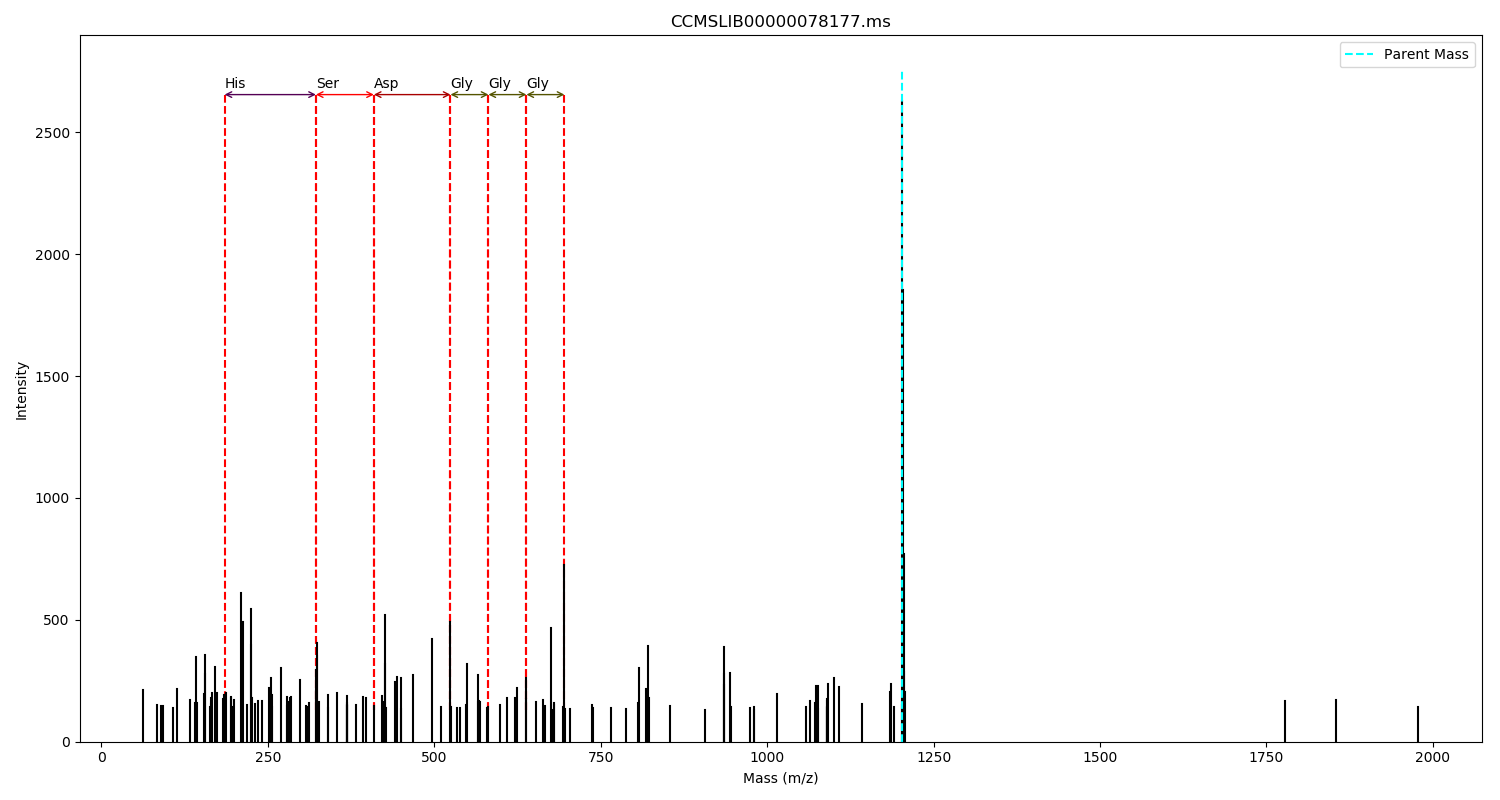
\includegraphics[width=1.0\linewidth]{images/spectragraph.png}}%

    \caption{An example plot of a detected length six tag above the mass-spectrometry readings for the molecule Cyclosporin in which it was found, generated using our Matplotlib-based accessory plotting tool. The tag His-Ser-Asp-Gly-Gly-Gly can be seen plotted along the peaks where it was found - the colours of the arrows used are tied to the label, and the user may provide a mapping from labels to colours. Note that this tag isn't necessarily correct - it's just an example of a visualisation of a tag arbitrarily chosen from the examples our algorithm found.}

    \label{fig:spectragraph}
\end{figure}

In practise, we implemented the NRP2Path scoring function with a few simplifying assumptions. Firstly, rather than utilising the statistical construction of the original authors for the prior probability, we instead assigned probability over the alphabet. Secondly, we implement only one of the two I-functions, the SVM I-function; the Stachelhaus Code I-function is not implemented. The prior probability as the original Pep2Path implements it is intended to estimate the probability of amino acids `in the wild' by treating the NORINE database as a representative sample of known information. This comes with the assumption, as the original authors note, that the distribution of amino acids in NORINE is generalisable, and indeed this may not hold for certain subcultures of bacteria or other contexts. Therefore, rather than bundling another layer of external complexity (dealing with NORINE data) with our implementation, we elected not to deal with this and instead provide simple implementations of tables of probabilities (implemented as a Python dictionary, again in the same way as the original Pep2Path) that can be swapped out as the end-user wishes as befitting their use-case.

For the I-functions, we were able to scrape the classes used to calculate the SVM I-function from the Pep2Path `database' file containing scores and from the implementation itself. \footnote{For an overview of how this is implemented, see Section \ref{nrpbackground}; for the full listing of classes, see Appendix \ref{svmclasses}.} For the Stachelhaus Code, however, we found that we couldn't easily reconstruct it, and would have to write our own implementation from scratch or directly integrate with NRPSPredictor2 or antiSMASH. Neither of these outcomes were desirable, so we instead parameterised I-functions as a list of functions (treating functions as first-class citizens i.e. data) and we leave this and any other novel I-functions open to future implementation. In both cases, we do not think these alterations will affect the overall behaviour of the score, just its accuracy in specific use-cases, so it suffices for our project aims.

One notable caveat is where the alphabet is concerned; the SVM method of course has a fixed alphabet, needing to know in advance how its various classes are constructed. When unknown components are used, it degenerates into evaluating \(1.0\) on an exact match and \(0.0\) otherwise; similarly we implement a 'prior probability' for any element which cannot be found in the Pdict as equal to the uniform probability of the elements contained. (This is not strictly speaking a probability, because while the elements in the Pdict sum to one, making them valid probabilities, adding any other component to this with a nonzero probability invalidates this. Since the probability is just a Bayes Rule inspired mechanism for calculating the score, and we do not need to rely on it having probabilistic properties, this shouldn't affect anything.)  We implement this this way so that it can generalise even to data with rare amino acids it doesn't know, but note that its performance will drop and it will not be appropriate for entirely unfamiliar datasets. Since we only calculate these values in order to compare them, this effectively 'factors out' the prior probability in lieu of more information about the population from which a sample originates.

Additionally, an important note is that our alphabet size is relatively small compared to the size of the data we are computing, so under normal circumstances, we would be continuously recomputing the values of functions between component matches. Instead, as the original Pep2Path does, we precompute a table of values, giving the values of all possible matches between two amino acids. In order to implement this, we use a nested dictionary structure, where when supplying a key to the external dictionary, in return we receive an internal dictionary which contains the other amino acid in the matching as a key, and the result of the function as the value. For the 20 proteinogenic amino acids, this is a table of 400 values - assuming they are 32-bit integers storing the values, approximately a kilobyte of memory is required to store the values in this table. (In practise, the table will be larger due to storing the dictionary structures and not just the values, but this gives an indication of the overall storage requirement.) Even if we had an alphabet size of 20000, storing the values requires approximately a gigabyte of storage space - a very reasonable requirement, given that this is unrealistically large!

On the other hand, precomputing the values like this means that there is some overhead at the start (constant-time with the number of input items) but allows us to avoid recomputing function values for the match between amino acids, using the O(1) time lookup of a hashmap. For an example of the alternative, we could naively implement the SVM class match by searching a component's amino acid class for the other amino acid in the matching; this is linear with the size of the class. While this is a small performance improvement - although wrapped inside the factorial-time of the alignment comparison - it generalises to more complicated functions. Therefore, we achieve better running times at a small space cost.

Furthermore one of our aims was the flexibility of the scoring system; in order to achieve this we wanted to have the ability to compose the scoring function's behaviour into the behaviour of larger functions i.e. the alignment comparison used in NRP2Path. The ability to pass around functions as first-class citizens makes this easy, but then the caller has to specify the parameters chosen. While we could have chosen to utilise variable arguments, this would then require each called function to parse its arguments, and any reader to infer the structure of those arguments; instead we chose to fix the argument list for each scoring function so that they could be called with the same fixed set of arguments; specifically a sequence tag and a set of Genbank predictions.

Having done this, however, each function would then have its own set of parameters that would need to be supplied to it in addition to the common operands. To solve this problem, we might use a factory method; a higher-order function which takes scoring-function-specific parameters, and emits a fixed scoring function adapted to the parameters given. This would allow us to compose the behaviour of the scoring function independently of the caller. However, there is one additional subtlety: because of our dictionary-based approach to computing I-values, we would then have to compose more behaviour onto this function (the matching dictionary) as it obtained information on the spectrum. Computing the lookup dictionary inside the function's scope would defeat the purpose of using it in the first place, and therefore we must compose behaviour onto the function from outside its scope. Therefore there must be some separate intermediary that the caller can access in order to be able to create the lookup dictionaries with the list of spectra it receives (we could also just give the function the original nested dictionary and let it recompute the match using this every time, but this would repeat some small computations, so instead we fix it to the components of a spectrum before passing it). However, this behaviour shouldn't be built-into the caller either; this would defeat our aim of composability. 

If we attempted to continue using higher-order functions we would have to awkwardly chain such fixers, complicating the design unnecessarily into various trees of subfunctions under each scoring function. It is for this reason we implement scoring functions as \textit{objects} and allow actual scoring to be done via a method built-in to the class. The class template is as follows: parameter behaviour is specified as the attributes of the object on object initialisation; other parameters needed at the start of each comparison (in our case the lookup dictionary) are defined by a setup method to which the spectrum and gene predictions are passed, but which otherwise relies on the object's internal state, unknown to the caller; finally we call the scoring method with the spectrum and gene predictions itself in order to compute a score. In this way we design a single interface for the calling of scoring functions (for example for alignment comparison), and composable behaviour packaged together within objects, whilst still not recomputing superfluous values on every call of the scoring function.

Therefore, we implement three linked components. First, the scoring class we described. Then, a single alignment comparing function, which compares a single spectrum to a single Genbank using the alignment comparison. Finally, a generalisation of this, which operates on a list of each and is given associated names - this is the implementation of the `many-to-many' comparison we mentioned in the requirements section. Currently, it only implements the capability to find the best score (and its associated names) and the average score, when scoring two groups against one another, but this could be extended to any other relevant features involved in scoring two groups against one another. The Jaccard scoring mechanism implements something similar.

Perhaps the most interesting detail of the implementation of the alignment comparison, however, is its direct mapping onto the Python Itertools module. Itertools provides a number of convenient functions generating iterators, which were used in numerous sections to simplify implementation, however, two of the most notable functions are itertools.permutations and itertools.product - which generate permutations and cartesian products specifically. These are exactly the mathematical constructs used in the alignment comparison, and by using them, we implement a large part of the alignment comparison in a mere three lines! (Three with the optimisation of not creating a tuple of forwards and backwards versions of symmetric assembly blocks; two otherwise.)

\begin{lstlisting}[language=python, float, caption={The three lines of code used to generate all possible assembly-orderings for the alignment comparison.}, label=lst:itertoolscode]
	mirror = lambda m : (m, list(reversed(m))) if (m != list(reversed(m))) else (m,)
	products = itertools.product(*[mirror(cds) for cds in gbk])
	orderings = [[comp for cds in ordering for comp in cds] for product in products for ordering in itertools.permutations(product, len(product))]
\end{lstlisting}

We also implement a few miscellaneous parsers required to get the data for the components. The spectral ones are diposable; they were quickly written for the files we had on hand. However, the Genbank parser was implemented for antiSMASH-produced Genbank files and should be usable with any files compliant with this format. In order to do this, we used a standard implementation provided by BioPython, a Python package defining biological utilities, and then filtered the useful information from it the data structure which it produced. This should ensure that unless the antiSMASH-produced Genbank file format is changed significantly, our parser should be as up-to-date as BioPython's standard implementation, and helps us manage this external dependency. We also use BioPython to translate frames in the six-frame translation of RiPP2Path.

Finally, we implement part of a CLI for the program - although it doesn't quite support running the program as a standalone, it does allow the running of several scripts, and provides a skeleton for the program to be used in this way.

\section{Performance} \label{performance}

Here we describe the empirical performance of our algorithms. The idea is not to give a precise benchmark (development and testing was performed on a relatively modest home machine - Intel Core i7-8550U Processor, 24GB RAM - where in practise we might use dedicated hardware) but rather to confront the algorithmic problems involved in development and attempt to measure a very rough timescale on which these algorithms perform in practise.

Despite its theoretical performance constraints, peptide sequencing performs unexpectedly well in practise. We tested with a real dataset of 5770 files, some of which had up to 20000 mass peaks before filtering for intensity. We found that it was able to identify sequence tags of up to length 6 with intensity filtering for peaks with < 5\% of maximum intensity in the spectrum, and a mass tolerance of \(0.01\), or filtering 0.5\% intensity and with a mass tolerance of \(0.001\) in under a minute. With settings of a filter threshold of 5\% and \(0.01\) mass tolerance, the program began to explore length 12 tags seemingly endlessly, and we did not check to see if it would terminate: in practise, we do not expect sequence tags to be this long, so the settings were likely unrealistic in any case. 

It is also worth noting that the runtime required was very unevenly distributed; most of it came from single, very large files (those with 20000 peaks). This is in line with what we would expect; in larger datasets, the worse than linear theoretical performance time becomes more of an encumbrance and stalls the entire process.

This gives us very optimistic projections for simpler datasets. However, it is worth noting that we used a mass table of only the proteinogenic amino acids for these results; these have quite varied masses (other than Leucine/Isoleucine, which we combined into a single entry in the mass table); in fact with the mass tolerances we used it is impossible for an edge to have more than one label (given that Leucine and Isoleucine are one label) so the running time must be coming almost entirely either from edge discovery or from constructing paths themselves and not alternative labellings - as we explained in \ref{msalgorithm} this is the \textit{easy} part of the problem. Under conditions where mass tables contain similar values, this algorithm is likely to be wholly inappropriate and another approach - for example the Antisymmetric Path Problem approach \cit{msbook} - should be used instead.

In practise, we found performance for RiPP2Path and the Jaccard Similarity to be very optimistic. RiPP2Path could process the entire genome of \textit{Streptomyces coelicolorA3(2)} with a sequence tag of length 8 in around half an hour to an hour. \textit{Streptomyces coelicolorA3(2)}'s genome contains approximately 9 million nucleobases; when run through the six-frame translation, this becomes approximately 3 million amino acids, and there are 6 frames, so we must compare approximately 18 million bases to our search tag - this is approximately 100 million character comparisons! This is on the order of \(10^8\), which is not too far off the number of clock cycles a modern processor has per second (ours is on the order of \(10^9\)), which, since these character comparisons are a little more complicated than a single clock pulse, suggests there's nothing glaringly inefficient about how we have implemented RiPP2Path.

For the Jaccard Similarity, we found that it could process all comparisons between the 5770 files mentioned earlier and a dataset of approximately 6000 Genbank files on the order of minutes, including time taken to parse these files. Therefore we can be assured of its performance in practise. However, the alignment-based comparisons are a little more complicated. Whilst they seemed to run indefinitely for the dataset we have just mentioned, they were capable of processing around 12000 spectra/BGC comparisons in order to produce the graphs used in Section \ref{scoregraphs} within a few minutes. There could be a number of factors at work here: for example, it may be possible that this comparison would terminate on an order of days or weeks due to it being a large dataset and a complicated comparison and we simply did not give it enough time (in practise we would expect to be computing smaller data on dedicated machines, so this is acceptable). It may also be the case that because the algorithm is factorial-time with the number of assembly-components, the real data simply has more assembly-components than the synthetic data we used to generate the graphs - we deliberately forced our generation to limit the number of assembly components so we could produce graphs in a reasonable amount of time, but future work might measure precisely the time taken with different assumptions about these components. Nonetheless, this is suggests our work is at least \textit{reasonably} performant.

However, the performance is less than ideal, so in future we might like to improve it. The most glaring bottleneck is the factorial-time (with tag-length) algorithm used for alignment; although it usually operates on very small data, this is an inefficient enough algorithm to potentially hugely hurt performance even on small data, and perhaps make solutions impossible for larger data. This is the number one area requiring attention in any performance-driven potential future development; see Section \ref{nrpalg} for more information.

Another possibility for improving the performance of NRP2Path would be to parallelise it, which is remarkably amenable to. For example, it would be easily possible to give each worker thread either a single pair of spectra and BGC to score, or a single ordering to score with the spectrum. This only offers performance linear with the number of non-virtual threads available, and is dependent on the hardware available where the larger problem is largely algorithmic, but due to the ease of parallelisation this is also a good next step.

Another issue of interest might be our language choice: whilst Python is very popular for its ease-of-use, it's not very performant - for example, one of its greatest strengths in portability and ease-of-use is the interpretated nature of the language. But this is also an Achilles' Heel - interpretation hurts performance significantly, due to the need to repeatedly fetch and decode instructions. For the absolute highest performance, we could rewrite the project in, say, C, or more realistically write certain underperforming portions in C and extend a wrapper around them from Python. However, this is a difficult and delicate process sacrificing many of the nice features of high-level languages, would sacrifice easy extension and would make any parts written in C maintainable only by a select group of rare experts. Even mid-level alternatives like Rust \cit{rustlang} and Julia would sacrifice the advantages we chose Python for. 

Fortunately, there exist a number of Python-based solutions to this problem. The first we have already mentioned; we could implement the performance-critical sections with C-based wrappers like NumPy, as we did for our MassSpectrum class. Although Scikit-learn \cit{sklearn} is a library for machine learning, it builds on NumPy and contains library functions for both Jaccard Similarity \cit{skjaccard} and Hamming Distance \cit{skhamming}; were we to change our data structures to accomodate these, we could potentially have performant and concise implementations of both. Other options include PyPy \cit{pypy} an alternative to the standard implementation of Python, CPython, supporting a Just-In-Time compiler which helps address the problems of interpretation - and Cython, a superset of the Python language with C-like features and a static compiler that boasts of performance on-par with C. Any of these solutions could offer a significant performance improvement (and potentially cleaner code), and some of them are relatively lightweight, so they too would make good next improvements.

Lastly, our tags (during the comparison stage) are implemented as lists of strings. We chose this implementation to allow the maximum flexibility in naming schemes for components, but a more efficient alternative might be to map names to fixed-length character sequences, and implement them as single strings. This would, however, require fixing an alphabet in advance (or generating an alphabet based on the character set in the data, but this brings its own set of challenges) and is unlikely to bring much of a performance improvement, so it is absolutely not a priority.

%==================================================================================================================================
\chapter{Evaluation} 

In order to ensure the correctness of our software, we describe in this chapter four methods of verification. Firstly, there is automated testing; this helps prove the correctness of our \textit{implementation} by testing certain invariants about the implementation. If the invariants are well-formulated, we will be able to demonstrate that the software implements what we intended to implement - but this does not necessarily prove that what we intended to implement was the \textit{correct} thing to implement. Nonetheless they are a useful internal diagnostic tool and eliminate most potential sources for error.

Secondly, our scoring functions are a central point of interest, so we perform an experiment and give the results here for the properties we wish to test about them. We do this for two reasons; while we know the properties of Jaccard Similarity and Hamming Distance \textit{a priori}, the NRP2Path scoring function is less amenable to analysis, so we demonstrate its empirical properties with the default settings instead. The other reason is that there is a particular emphasis on scoring functions; we would nonetheless have to use the same procedure when performing automated testing, but by describing this procedure and the results thereof we hope to illustrate clearly the behaviour of the scoring functions.

Thirdly, we detail the testing procedure for replicating the original Pep2Path experiments; such experiments will demonstrate:
\begin{enumerate}
	\item The empirical correctness of our implementation of Pep2Path (contingent on the correctness of the original implementation of Pep2Path).
	\item Performance on real-world datasets.
	\item The capacity for our platform to integrate outside scoring functions, such as the original NRP2Path scoring function (albeit with some 
		simplifications).
\end{enumerate}

Lastly, we examine how well our software met the original requirements we set out.

\section{Automated Testing}

For our automated testing, we test almost every function included in the software, and therefore have strong guarantees of the correctness of almost all components, provided the invariants we test are correct. In general, our procedure is to generate some data with a \textit{known} answer, add noise, and then check that the answer a function produces matches the correct answer. To illustrate this, the most notable examples are the tests for constructing sequence tags out of spectral data, and the tests for RiPP2Path.

For the sequence tags, we first randomly choose compounds from a provided mass table (the default is a mass table proteinogenic amino acids - the choice should be arbitrary) in random numbers, a random number of times. This gives us several random sequence tags, which we use as our 'true' values. We then convert these into masses, and compute consective cumulative sums between them in order to give us ordered mass peaks with mass gaps corresponding to our true results. We then add some completely random mass peaks, filter out any duplicates and add noise to every peak equal to half the mass tolerance, chosen arbitrarily to be \(0.001\) (since we are looking for differences, it is necessary to give use half the mass tolerance lest the errors 'double up' between the two peaks involved in a difference). We then check that the the tags found from this data contain the original 'true' tags as a subset (by random coincidence there may be generated other generated tags - especially if the mass tolerance were high).

For RiPP2Path we perform a similar procedure. We don't test the entire process end-to-end - we only test the scoring portion, once the two tag and genome comparable format (i.e. we assume we have the six-frame translation as given, rather than generating a DNA sequence - in order to generate true data within a DNA sequence, we'd have to reverse-engineer BioPython's translation). First we generate a true tag. Then, we embed it in a few thousand generated characters from the alphabet, using this as our first frame; for the other five, we repeat this process without a 'true' tag. We then receive the scores from RiPP2Path, filter them for perfect scores, and check that any of the returned perfect scores (in case we generated the same one by chance) have the location we inserted the 'true' tag at, the correct strand and are the same tag.

This procedure isn't perfect and is dependent on the invariants - for example at one point the RiPP2Path test was filtering for all scores equal to the top score, and would return a pass if, for example, RiPP2Path returned uniform scores - but it builds the correctness of various small components up and taken together with our other results gives a good indication that our software is correct.

\section{Scoring Functions} \label{scoregraphs}

There are three properties of our scoring functions we would like to demonstrate:
\begin{enumerate}
	\item That the function is bounded above by the score for an exact match.
	\item That the function is generally decreasing as we move further away from an exact match.
	\item That the function is proportional; i.e. if the tag being compared is longer, then a mismatch causes a larger drop in score than it would for a 		shorter tag.
\end{enumerate}

In order to test these properties, we designed the following experiment. We start with an identical sequence tag and set of genbank predictions. Then we want to repeatedly randomly mutate one of these (the choice should be arbitrary; we choose to mutate the sequence tag because it's slightly easier to implement) and measure the score as we do so. This should be sufficient to demonstrate properties one and two - if we plot the results, we should see that the highest point is the first value, and that the graph trends down towards some baseline. In order to demonstrate property 3, we need to repreat this procedure multiple times for multiple different tag lengths and compare how many mutations it takes for the function to approximately reach its baseline (note that this process is random, so the basal value we converge to may be different).

To carry out this procedure, firstly, we generate a synthetic sequence tag from a given alphabet. Then, we create an exact copy for for the Genbank predictions, which we partition at random into smaller blocks analogous to NRPS modules, rearrange these modules and for each module choose at random whether it should be reversed or not. This creates a set of Genbank predictions which is expected to be identical, and tests the rearrangement portions of scoring function for the alignment-based scoring functions. We then measure the score between these two pieces of synthetic data.

From this set of genbank predictions, we generate \(b\) mutants, where \(b\) is an arbitrary parameter defining batch size.  A mutant of a tag is the tag with one randomly-chosen component replaced by another randomly-chosen component from its alphabet with uniform probability (it may be the same one; it depends on the size of the alphabet chosen, but we repeat this process so it should in general converge to produce mismatches). Then at each time step, we take the previous batch of mutants, and mutate them again to produce a set of mutants which randomly move progressively further from being a total match. We then plot these data. 

For this procedure, there are four parameters: \textit{alphabet}, \textit{batch size}, \textit{number of mutations} and \textit{tag length}. \textit{Alphabet} defines the components we can draw from when randomly generating both the original tags and mutants; in general, this should have little effect other than that a small alphabet would have greater chance (with uniform probability) to draw the same amino acids repeatedly, and hence this procedure would not converge easily. For our experiments, we simply use the alphabet of proteinogenic amino acids.

\textit{Batch size} defines how many mutants are generated at each stage. In order to make the trend clearer, we average the score of the mutants in each batch, and plot each average score as an individual point. So in general as batch size increases, these points should converge to their 'true' expected score values for that many mutations, and the graph should get 'smoother'. We try to use batch values of at least a few points and higher where we can, but there is an associated linear performance cost to doing so.

The \textit{number of mutations} controls the total number of batches of mutations we generate; this must be long enough enough that we generate enough mutations to see the score decay to some baseline (and stay there), but it again has an associated linear performance cost. In general we aim for 100 mutations, which suffices to see the whole decay for shorter tags. We also attempt to keep this and batch size fixed within experiments conducted on a single scoring function, and fix the bottom of the axis to 0, for ease of comparison.

\textit{Tag length} is simply the length of the tags (and all subsequent mutants) that we generate. This is necessary to demonstrate property 3; we vary this to see the decrease in score. It's worth noting that the proportionality effect will be compounded by the fact that as a tag gets longer, when choosing which component to mutate, then over time it is increasingly likely we will choose an element that we have already mutated, and thus is likely to already be a mismatch, and so our position in the tag space does not meaningfully move away from perfect match. In other words, for longer tags we are likely to take longer to converge at baseline and may converge at a higher point not only because of the result we expect, but also due to \textit{a bias in the testing procedure}. 

This doesn't make our testing procedure infeasible, however; this effect becomes more pronounced as we go through more mutations, whereas proportionality should be observable throughout. We can determine if a scoring function is proportional by checking its behaviour \textit{at the start} and seeing how quickly it decays. In fact, while this effect becomes more pronounced overall for longer tags, it is \textit{less} pronounced towards the start, due to the fact that we are much more likely to pick a new component to mutate - it is only \textit{convergence} behaviour it affects, and this doesn't come into question for property 3. (And we are concerned with property 2 independently of tag length.)

Alternatively, another experimental design would be to choose which component to mutate next deterministically, or to choose randomly but only choose components that haven't already been mutated. However, an exhaustive search of the scoring space is impossible - or at least very computationally expensive for longer tags, as it will be exponential with the size of the alphabet - so to take these approaches would be to encode certain assumptions about the order we perform mutations in. This bias is unlikely to matter, but we choose to avoid it in favour of exploring the scoring space more randomly at the cost of having a more meandering procedure. We \textit{do} still encode these assumptions to a certain extent by iteratively mutating the same group of mutants, but this enables us to 'walk' the scoring space, and have each group of mutants immediately comparable to the previous, so it is an acceptable compromise here.

\begin{figure} \label{fig:jaccards}
    \centering
    \makebox[\linewidth][c]{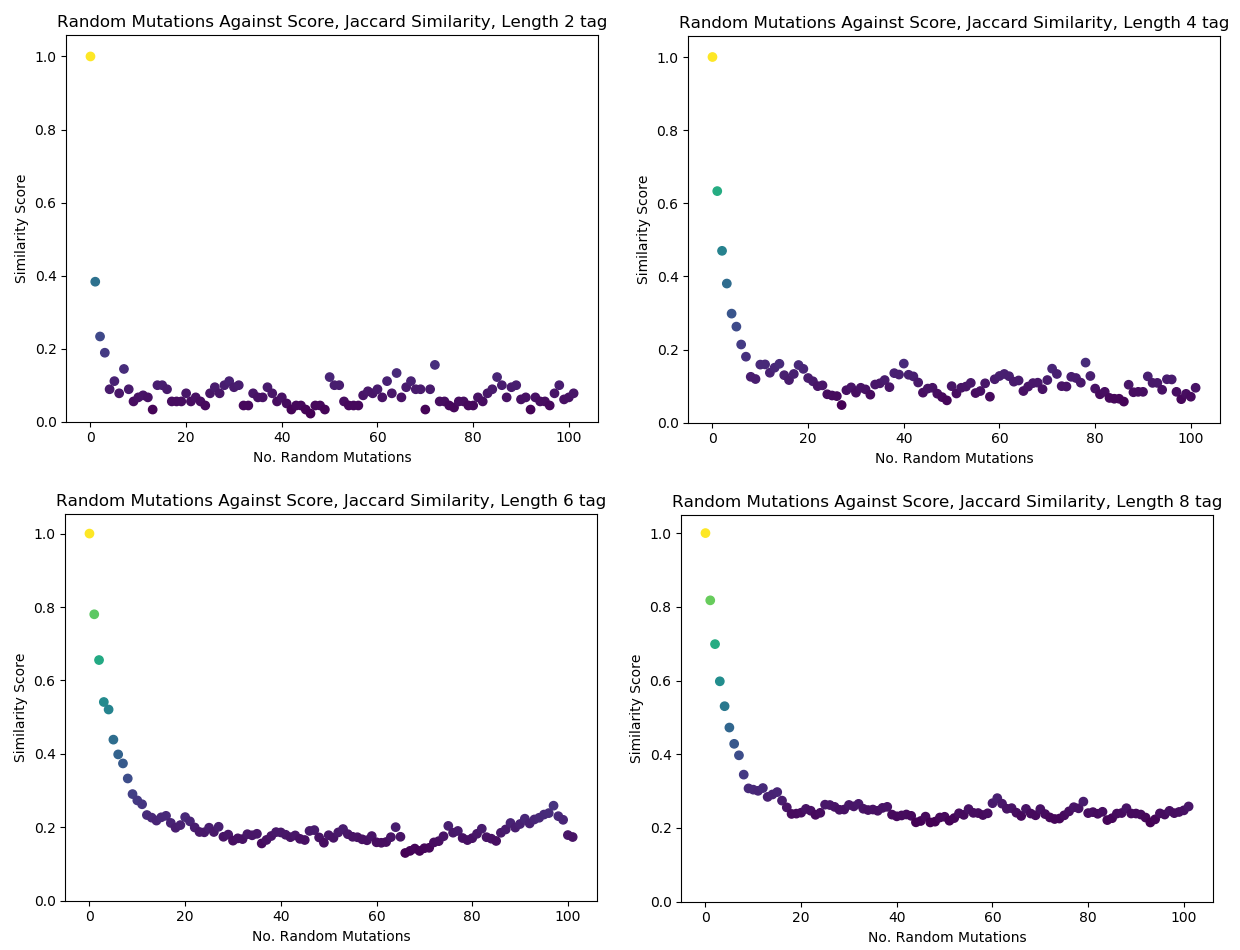
\includegraphics[width=1.0\linewidth]{images/jaccards.png}}%

    \caption{Four plots of Jaccard Similarity for different tag lengths.}

    \label{fig:jaccards}
\end{figure}

\begin{figure} \label{fig:jaccard20}
    \centering
    \makebox[\linewidth][c]{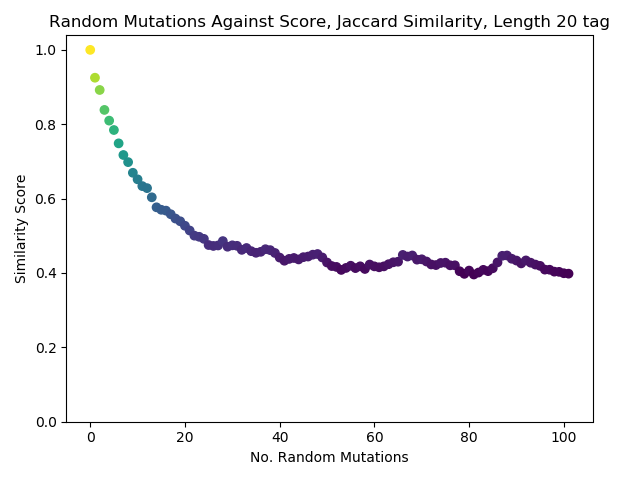
\includegraphics[width=1.0\linewidth]{images/jaccard20.png}}%

    \caption{An extended plot of Jaccard Similarity, for a length 20 tag. In general this is an unrealistically long tag, but we extend the scoring function in order to show the general trend more clearly.}

    \label{fig:jaccard20}
\end{figure}

\begin{figure} \label{fig:simples}
    \centering
    \makebox[\linewidth][c]{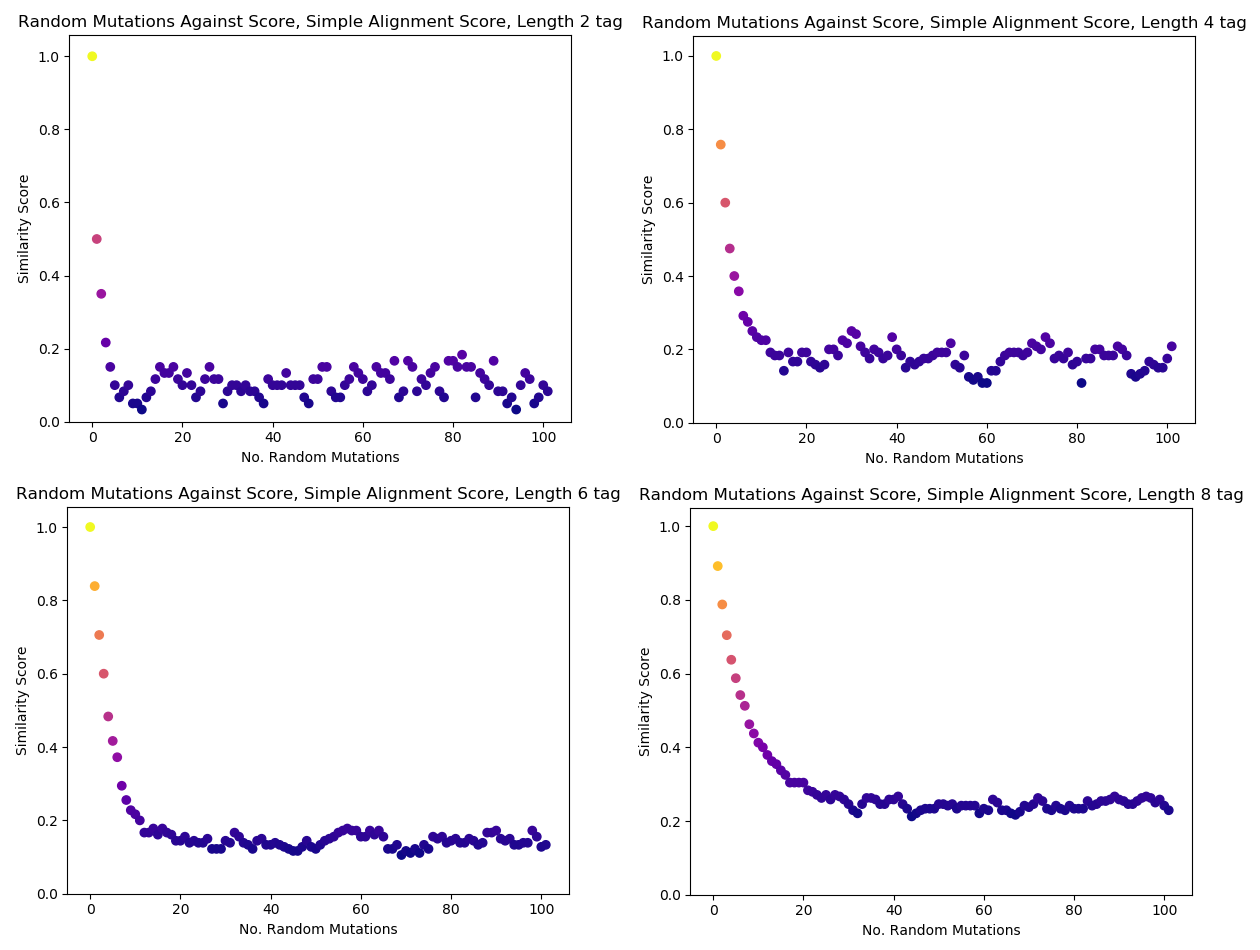
\includegraphics[width=1.0\linewidth]{images/simples.png}}%

    \caption{Four plots of the alignment comparison with the simple Inverse Normalised Hamming Distance score for different tag lengths.}

    \label{fig:simples}
\end{figure}

\begin{figure} \label{fig:p2ps}
    \centering
    \makebox[\linewidth][c]{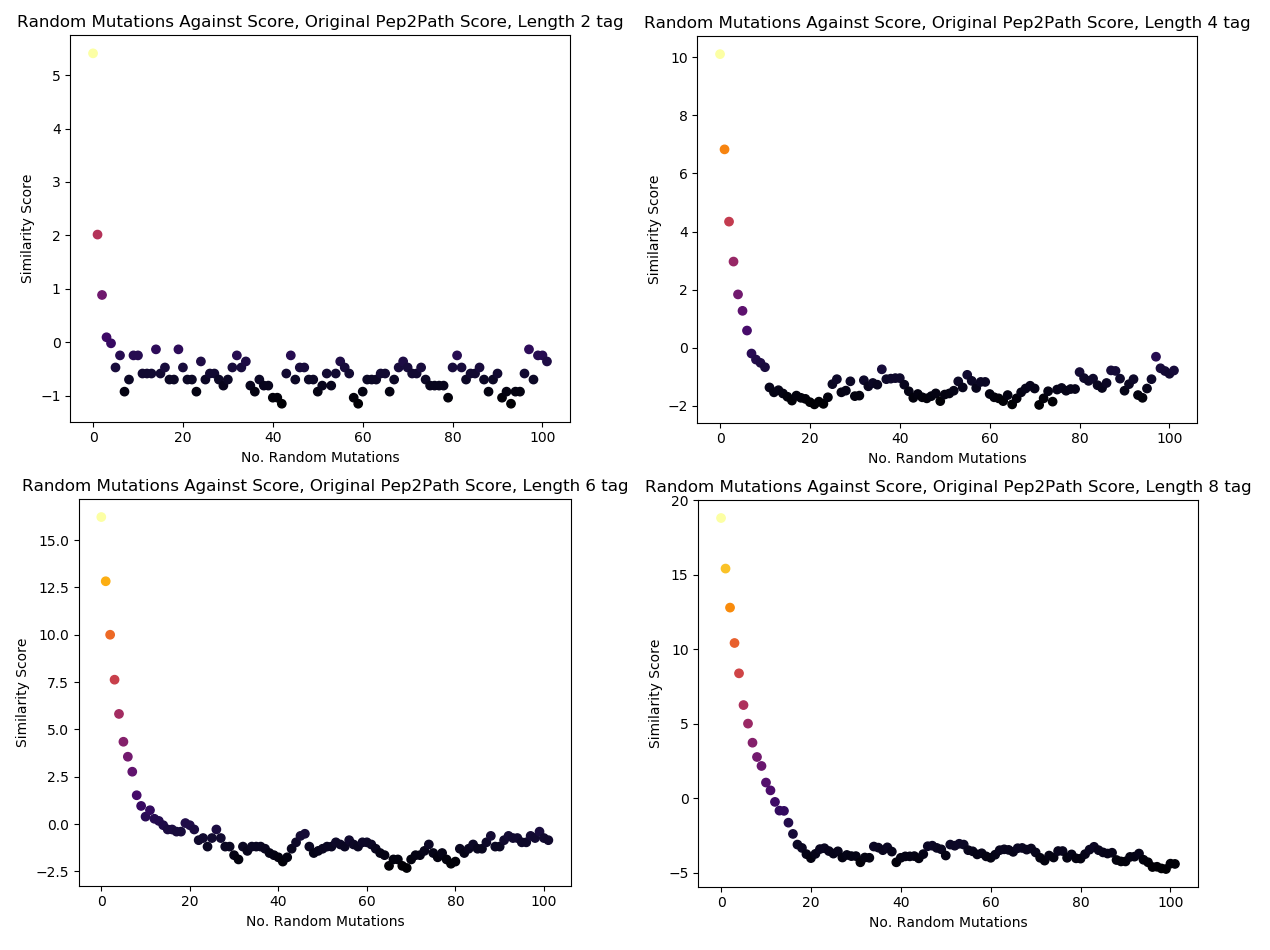
\includegraphics[width=1.0\linewidth]{images/p2ps.png}}%

    \caption{Four plots of the alignment comparison with the original NRP2Path score for different tag lengths.}

    \label{fig:p2ps}
\end{figure}

Note also that checks on these properties can be implemented by means of automated testing for the scoring functions; we implement a check on property 1 by performing the iterative mutation process, taking the scores sorted in non-decreasing order by number of mutations, and then use a sorting algorithm to sort in non-increasing order of score; the first value should be the score for no mutations in this case. It would also be possible to enforce properties 2 (by iteratively generating certain mismatches in the tag and checking if the score decreases) and 3 (by performing the same process but instead comparing the drops in score between tag lengths as mismatches are added) but we do not currently implement these at this time for the reasons we outlined at the start of this chapter.

\section{Original Pep2Path Experiments}

To implement the original Pep2Path experiments, the authors of the original paper helpfully provided exact instructions for how to perform their experiments with their software in one of their supplementary documents (available with their original paper). This is done by running a command - all their data is bundled with their software, so running their experiments is a matter of downloading it and accessing their database file and Genbank files. (The original Pep2Path does not concern itself at all with Mass Spectrometry.) By performing these experiments, we prove both that we have reimplemented the original software and also allow its results to be generalised to our software.

For Ripp2Path, we produced the results seen in Figure \ref{fig:ripp2path} by searching for the tag VHFVGW[I,L] inside the entire genome of \textit{Streptomyces coelicolorA3(2)}. The top three are identical to those of the original authors' results; the next seven share scores, but are different; this is probably due to a slightly different sorting order and so we can say we have successfully replicated the results of the original paper in this case.

\begin{figure} \label{fig:ripp2path}
    \centering
    \makebox[\linewidth][c]{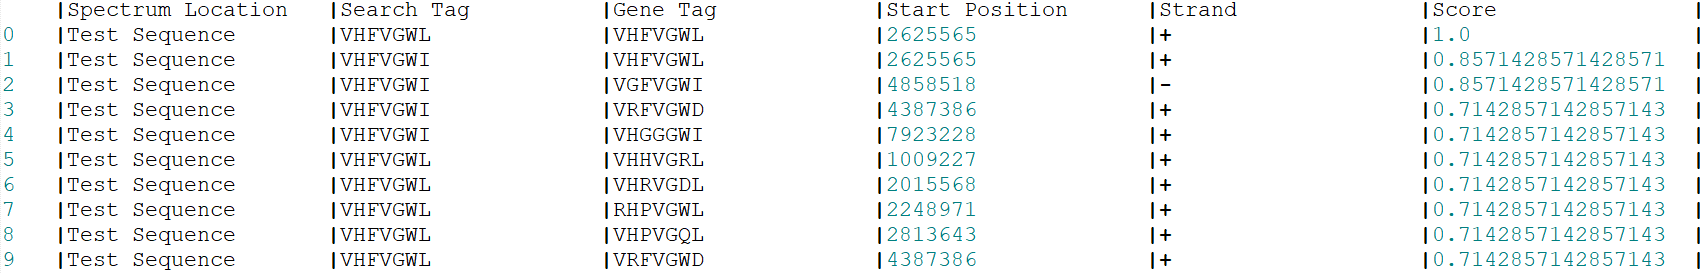
\includegraphics[width=1.0\linewidth]{images/ripp2path.png}}%

    \caption{A screenshot of part of the  table of results the RiPP2Path algorithm produced searching for the tag VHFVGW[I,L] inside the Streptomyces coelicolorA3(2) genome.}

    \label{fig:ripp2path}
\end{figure}

Regretfully, we were not able to collect the original results for NRP2Path within the time we had - any such experiment would have to process the massive NORINE database multiple times and our timeframe was limited. Any interested party may adapt our implementation to the instructions of the original authors: the only point of note is that the original Pep2Path's distribution comes with a `database' file defining antiSMASH 2 predictions for everything in the NORINE database; these can be extracted, and used to calculate the NRP2Path score. 

\section{Fulfilment of Project Requirements}

Firstly, the project we have described it has fulfilled all of the `Must Have' requirements from our MoSCoW model of the requirements, (see Section \ref{moscow}) so it is a success in this regard. Under `Should Have' we implement both RiPP2Path and the `many-to-many' comparisons; as we have just seen, we do not provide all of the original experimental results, but the possibility is there for anyone who wishes to test, and we believe we have sufficient correctness guarantees that this is a minor point. The code has not yet been integrated with the client's codebase, but is scheduled to be delivered, so, again, we do not consider this a failure. Under 'Could Have' we implement the accessory plotting tool and a partial CLI, but do not implement adopt part of the RiPPQuest method. However, since the essential requirements are covered and everything other than one 'Could Have' requirement is covered, functionally we can say this project satisfies the requirements.

Non-functional requirements are a little more subjective and complicated - unfortunately, in order to address some of these, we have no choice but to put forth our personal opinions! Both platform-independence and the use of established tools to facilitate accessibility to outside experts follow from the fact that we used Python for our implementation, and other than this and a few packages installable with PIP, have no direct dependencies. For efficiency - some of the software operates on large datasets in reasonable time, and all of it achieves the same with more modest datasets, even on a regular laptop. Therefore, we feel confident in concluding that it is efficient enough to be practical, if not necessarily optimal, which was our main requirement. We also feel that we have sufficiently encouraged component reuse by separating our design into several packages - users can, for example, switch out the Mass Spectrometry package for a more sophisticated one and still take advantage of our implementation of Pep2Path. Finally, clarity of design is really up to the discretion of whoever happens to be studying it; but given our adherence to the design principles we outline in Section \ref{implementation} and that, as an example, the body of one of our main algorithms can be expressed as cleanly as in \ref{lst:itertoolscode} we hope you will agree with us that our design, while not perfect, is sufficiently clear.

%==================================================================================================================================
\chapter{Conclusion}    

\section{Summary}

In conclusion, we have implemented a piece of software that implements the functionality of the original Pep2Path. We:
\begin{itemize}
\item Outline its motivation as a piece of software to match mass spectrometry data to biosynthetic gene cluster predictions, in order to automate the identification of natural products and aid the drug identification pipeline.
\item Describe its design, examining its architecture and closely analysising the algorithms used and their performance.
\item Describe the implementation, including language choice, the software design practises we aimed to follow and the performance of our software with respect to computational time, offering future suggestions for improving it.
\item Demonstrate the correctness of this software by several methods: automated testing, experiments with the behaviour of scoring functions used and by partial replication of the original experiments used to demonstrate the correctness of its predecessor.
\end{itemize}

Overall, our algorithms match those presented in Pep2Path, with some minor simplifications to NRP2Path. Our results show that our implementation of RiPP2Path matches that of the original Pep2Path, and our automated testing gives us strong indications of correctness on all other fronts. Additionally, our experiments with our scoring mechanisms shows that in general they provide useful scores, by assigning the best score to a perfect match and generally decreasing scores as one moves away from a perfect match, and mismatches penalise scores proportionally to how significant the mismatch is within the overall context. Our implementations also run in reasonable time (we do not provide precise benchmarks - they are not especially important) - on the order of minutes for most cases, and approximately an hour on large data in one case. Only NRP2Path seemed to fail to terminate when given hours to do so, and only when being run on very large data. We also implement this software in adherence with software design practices, and therefore hopefully provide software that is clean, concise and maintainable.

\section{Future Work}

For future work, there are three main points we think are important: \textbf{Correctness}, \textbf{Performance} and \textbf{Extension}.

\begin{itemize}
\item \textbf{Correctness:} So far we have demonstrated the broad correctness of our software via \textit{controlled experiments} on \textit{synthetic data} via the automated testing and scoring experiments. There are a few miscellanea in this area still to be addressed; for example it might be useful to implement the other suggestions for automated testing we outline in Section \ref{scoregraphs}. However we think the priority in this region is to begin running \textit{natural experiments} on real data and get empirical feedback from the real world. The first step in this process would be to complete the rest of the Pep2Path experiments; but there may be other datasets for which this would be helpful. It may also be helpful to integrate Pep2Path v2 with a more sophisticated mass spectrometry module, so that we don't fall prey to ``Garbage In, Garbage Out" - Pep2Path depends on these inputs.
\item \textbf{Performance:} Our algorithms in general perform well in terms of running time, but NRP2Path in particular is limited to not being able to complete its work on larger datasets. The most important factor in this by our estimation is to improve the factorial-time algorithm - but we suggest many other algorithmic improvements in Section \ref{algorithms} and more software-oriented suggestions in Section \ref{performance}. It may also be useful to get precise benchmarks for performance, especially as we vary the number of assembly-blocks in a Genbank prediction - this is likely to be where the largest bottleneck lies.
\item \textbf{Extension:} Our work is far from complete! There are many other directions which this software could be taken - for example, it could utilise RiPPQuest-like methods (see Section \ref{ripps}) or implement new scoring functions, such as the Levenshtein distance. Our work is largely informed from the original paper and the computer science and software development end of things - there are likely to be many improvements that could come from biochemistry!
\end{itemize}

%==================================================================================================================================
%
% 
%==================================================================================================================================
%  APPENDICES  

\begin{appendices}

\chapter{Appendices}

\section{Classes Used in SVM I-Function} \label{svmclasses}

%\begin{adjustbox}{width=0.9\textwidth}
\begin{lstlisting}[language=python, float, caption={Classes used for SVM-I Function. Any exact match evaluates to 1.0. A small-class match evaluates to 0.75, a large-class match evaluates to 0.5, a three-class match evaluates to 0.25, and it evaluates to 0 otherwise.}, label=lst:svmclasses]
svm_alphabet = ['ala', 'gly', 'val', 'leu', 'ile', 'abu', 'iva', 'ser', 'thr', 'hpg', 'dhpg', 'cys', 'pro', 'pip', 'arg', 'asp', 'glu', 'his', 'asn', 'lys', 'gln', 'orn', 'aad', 'phe', 'tyr', 'trp', 'dhb', 'phg', 'bht']
		
three_classes = {'hydrophobic-aliphatic':['ala', 'gly', 'val', 'leu', 'ile', 'abu', 'iva', 'ser', 'thr', 'hpg', 'dhpg', 'cys', 'pro', 'pip'],
                 	 'hydrophilic':['arg', 'asp', 'glu', 'his', 'asn', 'lys', 'gln', 'orn', 'aad'],
                 	 'hydrophobic-aromatic':['phe', 'tyr', 'trp', 'dhb', 'phg', 'bht']}

big_classes = ['gly,ala,val,leu,ile,abu,iva',
			   'ser,thr,dhpg,hpg', 
			   'asp,asn,glu,gln,aad', 
			   'dhb,sal', 
			   'cys', 
			   'phe,trp,phg,tyr,bht', 
			   'orn,lys,arg', 
			   'pro,pip']

small_classes = ['val,leu,ile,abu,iva', 
				 'ser', 
				 'gly,ala', 
				 'dhb,sal', 
				 'cys', 
				 'thr', 
				 'asp,asn', 
				 'phe,trp', 
				 'glu,gln', 
				 'pro', 
				 'tyr,bht', 
				 'orn,horn', 
				 'dhpg,hpg', 
				 'arg', 
				 'aad']
\end{lstlisting}
%\end{adjustbox}

\end{appendices}

%==================================================================================================================================
%   BIBLIOGRAPHY   

% The bibliography style is abbrvnat
% The bibliography always appears last, after the appendices.

\bibliographystyle{abbrvnat}

\bibliography{l4proj}

\listoffigures

%\listoftables

\end{document}
